% !TEX program = xelatex
\documentclass[UTF8,fontset=fandol,a4paper,11pt]{ctexart}
\usepackage[margin=21mm,top=23mm,bottom=22mm,headheight=16pt]{geometry}
\usepackage{amsmath,amssymb,mathtools,bm}
\usepackage{tikz}
\usetikzlibrary{arrows.meta,calc,angles,quotes,patterns}
\usepackage{xcolor,booktabs,array,longtable,enumitem,fancyhdr,needspace}
\usepackage[unicode,hidelinks]{hyperref}
\definecolor{ink}{HTML}{24343C}
\definecolor{accent}{HTML}{166A70}
\definecolor{muted}{HTML}{65747A}
\definecolor{rulegray}{HTML}{D4DDE0}
\definecolor{warm}{HTML}{966037}
\color{ink}
\setlength{\parindent}{2em}
\setlength{\parskip}{4pt}
\linespread{1.12}
\AtBeginDocument{\setlength{\abovedisplayskip}{6pt plus 2pt minus 1pt}
\setlength{\belowdisplayskip}{6pt plus 2pt minus 1pt}
\setlength{\abovedisplayshortskip}{0pt plus 1pt}
\setlength{\belowdisplayshortskip}{4pt plus 1pt}}
\setlist[enumerate]{label=(\arabic*),leftmargin=2.3em,itemsep=3pt,topsep=4pt}
\setlist[itemize]{leftmargin=2em,itemsep=2pt,topsep=4pt}
\allowdisplaybreaks[1]
\setlength{\emergencystretch}{2em}
\setcounter{secnumdepth}{0}
\providecommand{\tightlist}{\setlength{\itemsep}{0pt}\setlength{\parskip}{0pt}}
\ctexset{section={format=\Large\bfseries\color{accent},beforeskip=10pt,afterskip=9pt},
subsection={format=\normalsize\bfseries\color{accent},beforeskip=10pt,afterskip=4pt},
subsubsection={format=\normalsize\bfseries,beforeskip=8pt,afterskip=3pt}}
\pagestyle{fancy}
\fancyhf{}
\fancyhead[L]{\small\color{muted}物理学难题集萃}
% 页眉仅保留书名；版本名称只在封面显示。
\fancyfoot[L]{\small\color{muted}\chapterlabel}
\fancyfoot[R]{\small\thepage}
\renewcommand{\headrulewidth}{0.4pt}
\renewcommand{\footrulewidth}{0pt}
\newcommand{\dd}{\mathop{}\!\mathrm{d}}
\newcommand{\vect}[1]{\bm{#1}}
\newcommand{\tagline}[1]{\noindent{\small\color{muted}#1}\par}
\newcommand{\result}[1]{\begin{equation*}\boxed{#1}\end{equation*}}
\newcommand{\figcaption}[1]{\par\vspace{2pt}{\small\color{muted}#1}\par}
\newcommand{\teach}[2]{\Needspace{4\baselineskip}\subsection*{讲解要点与追问}#1\par\smallskip\noindent\textbf{追问：}#2\par}
\newcommand{\workarea}{\par\vspace{7mm}\noindent{\small\color{muted}作答区}\par\vspace{4mm}
\noindent\textcolor{rulegray}{\rule{\linewidth}{0.3pt}}\par\vspace{16mm}
\noindent\textcolor{rulegray}{\rule{\linewidth}{0.3pt}}\par\vspace{16mm}
\noindent\textcolor{rulegray}{\rule{\linewidth}{0.3pt}}\par\vspace{16mm}
\noindent\textcolor{rulegray}{\rule{\linewidth}{0.3pt}}}
\tikzset{axis/.style={-{Stealth[length=2mm]},thin,color=muted},
motion/.style={-{Stealth[length=2.3mm]},thick,color=accent},
force/.style={-{Stealth[length=2.3mm]},thick,color=warm},
traj/.style={thick,color=accent},guide/.style={dashed,thin,color=muted},
object/.style={thick,color=ink},every node/.style={font=\small}}\widowpenalty=10000\clubpenalty=10000\displaywidowpenalty=10000\newcommand{\chapterlabel}{综合试题（一）}







\hypersetup{pdftitle={综合试题（一）·学生解答版},pdfauthor={}}

\begin{document}\pdfbookmark[0]{综合试题（一）}{cover}

\thispagestyle{empty}\vspace*{22mm}

\noindent{\Huge\bfseries 物理学难题集萃}\par\vspace{12mm}

\noindent{\LARGE 综合试题（一）}\par\vspace{12mm}

\noindent{\Large\color{accent}学生解答版}\par\vspace{9mm}

\noindent\textcolor{accent}{\rule{\linewidth}{1pt}}\par\vspace{9mm}

\noindent 第1--6题\par\vfill\clearpage

\pdfbookmark[1]{题目目录}{contents}\section*{题目目录}

\begin{longtable}{@{}r p{113mm} r@{}}\toprule 题号 & 题目 & 页码\\\midrule

\hyperref[q:1]{1} & \hyperref[q:1]{内盘与外环的两阶段摩擦运动} & \pageref{q:1} \\

\hyperref[q:2]{2} & \hyperref[q:2]{椭圆轨道的引力规律与彗星速度} & \pageref{q:2} \\

\hyperref[q:3]{3} & \hyperref[q:3]{四维理想气体的统计规律和热过程} & \pageref{q:3} \\

\hyperref[q:4]{4} & \hyperref[q:4]{三个频率电源的稳态电流与平均功率} & \pageref{q:4} \\

\hyperref[q:5]{5} & \hyperref[q:5]{幂律径向电场中的粒子束聚焦} & \pageref{q:5} \\

\hyperref[q:6]{6} & \hyperref[q:6]{列车入隧道与机械扰动的传播} & \pageref{q:6} \\

\bottomrule\end{longtable}

\clearpage

\pdfbookmark[2]{第 1 题 内盘与外环的两阶段摩擦运动}{q1}

\section*{第 1 题\quad 内盘与外环的两阶段摩擦运动}\label{q:1}


从半径$2R$的均匀薄圆盘中央切出半径$R$的圆盘，切缝很窄，得到质量$m$的内盘和质量$3m$的外环。二者竖立于水平地面，初始共同向右平动，速度$v_0$，均不转动。外环与地面间滑动摩擦因数$\mu_0=0.5$，内盘与外环间滑动摩擦因数为$\mu$，静摩擦的最大比值也取$\mu$；地面静摩擦上限取$0.5$倍法向力。重力加速度$g$。

忽略窄缝造成的两圆心位移及接触点迁移的短暂过程，视为两圆心有相同水平加速度，竖直位置不变。
\begin{enumerate}
\item 求内盘与外环间出现相对滑动的$\mu$范围。
\item 取$\mu=0.2$，讨论地面由滑动变为无滑滚动前后的运动，求最终共同平动速度。列出两阶段加速度及转换条件，并检查地面静摩擦是否足够。
\end{enumerate}


\begin{center}\begin{minipage}{.98\linewidth}\centering
\begin{tikzpicture}[scale=.8,transform shape]

\draw[object] (0,0) circle (2); \draw[object] (0,0) circle (1.03);
\draw[object] (0,0) circle (.98);
\draw[object] (-3,-2)--(3.8,-2);
\fill (0,0) circle (1.5pt) node[above left] {$O$};
\draw[guide] (0,0)--(45:2) node[pos=.82,above left] {$2R$};
\draw[guide] (0,0)--(-35:1) node[midway,above] {$R$};
\node at (-.4,.5) {$m$};\node at (-1.45,.5) {$3m$};
\draw[motion] (2.4,.6)--(4.3,.6) node[right] {$v_0$};
\node[below] at (0,-2.2) {地面：$\mu_0=0.5$};
\node[align=left] at (6.3,-.3) {内接触：$\mu$\\初始两者均不转\\切缝与中心位移略去};

\end{tikzpicture}
\figcaption{图综一.1\quad 外环外半径2R，内盘半径R；最初共同平动。}
\end{minipage}\end{center}

\Needspace{6\baselineskip}\subsection*{解答}


先按两个接触面的相对速度安排运动过程。地面上的接触点位于外环最下端，向右速度为$u_g=v-2R\omega_2$。内盘与外环的圆心以相同速度平移，所以内接触处的相对切向速度只由转动差给出，大小为$u_i=R(\omega_2-\omega_1)$。初始$u_g=v_0>0$，地面摩擦向左，给外环顺时针力矩；内摩擦再带动内盘顺时针旋转。内摩擦较小时，外环先转得较快，两个接触面都发生滑动。地面滑动消失时，内接触仍保留转速差，随后进入外环滚动、内接触滑动的第二阶段。这样每次转换都对应一个明确的速度等式。

图综一.1中外半径为$2R$，内接触半径为$R$。两部分的转动惯量为
\[
I_1=\frac12mR^2,\qquad
I_2=\frac12(3m)[(2R)^2+R^2]=\frac{15}2mR^2.
\]
统一取顺时针角速度为正，向右平动速度为$v$，减速度大小为$a=-\dot v>0$。内盘竖直加速度为零，内接触合力为$(-ma,mg)$；它的法向分量$N_1$和切向摩擦$f_1$互相垂直。在内接触滑动、外环转得较快的阶段，
\[
f_1=\mu N_1,\qquad N_1^2+f_1^2=m^2(a^2+g^2),
\]
因此
\[
\boxed{N_1=\frac{m\sqrt{a^2+g^2}}{\sqrt{1+\mu^2}},
\quad f_1=\frac{\mu m\sqrt{a^2+g^2}}{\sqrt{1+\mu^2}}}.
\]
把接触合力记为$\boldsymbol F_1$。内盘竖直位置不变，因此$F_{1y}=mg$；水平方向以加速度$-a$运动，因此$F_{1x}=-ma$。这两个分量确定合力，接触法线沿接触半径，切向摩擦与其垂直。三者构成直角三角形，$F_1^2=N_1^2+f_1^2$，再代入$f_1=\mu N_1$便得到支持力和摩擦力。外环受到大小相等、方向相反的内接触力，其竖直向下分量为$mg$，所以地面正压力同时承担两部分的重量。

接触点的位置也可由这个力三角形给出。令$A=a/g$，$\boldsymbol n$为作用在内盘上的法向单位矢量，切向单位矢量为$\boldsymbol t=(-n_y,n_x)$。由$N_1(\boldsymbol n+\mu\boldsymbol t)=mg(-A,1)$，解得
\[
\boldsymbol n=\frac{(\mu-A,\ 1+\mu A)}{\sqrt{(1+A^2)(1+\mu^2)}},\qquad
\frac{\boldsymbol r_P}{R}=-\boldsymbol n.
\]
其中$P$为内接触点。第一阶段$A=0.5,\mu=0.2$时，$\boldsymbol r_P/R\simeq(0.2631,-0.9648)$；第二阶段$A\simeq0.01669$时，$\boldsymbol r_P/R\simeq(-0.1797,-0.9837)$。两图分别按各阶段的力平衡画接触方向。窄缝使接触点在转换附近迅速迁移，题设近似把迁移的短暂过程略去，各阶段仍分别采用相应的定常接触方向。

接触法线随合力的水平分量倾斜，支持力由合力和摩擦的直角分解求出。
\begin{center}\begin{minipage}{.98\linewidth}\centering
\begin{tikzpicture}[scale=.8,transform shape]

\draw[object] (0,0) circle (1.3);
\coordinate (P) at (.342,-1.254);
\fill (P) circle (2pt);
\draw[force] (P)--(-.08,.30) node[above] {$N_1$};
\draw[force] (P)--(-1.10,-1.65) node[left] {$f_1$};
\draw[force] (0,0)--(0,-1.9) node[below] {$mg$};
\draw[motion] (-1.6,1.7)--(-2.8,1.7) node[left] {$a_1$};
\draw[guide] (0,0)--(P);
\node at (0,2.6) {内盘：顺时针力矩$Rf_1$};
\begin{scope}[xshift=6cm]
\draw[object] (0,0) circle (2); \draw[object] (0,0) circle (1);
\draw[force] (0,-2)--(-1.7,-2) node[left] {$f_2$};
\draw[force] (0,-2)--(0,-.5) node[right] {$N_2$};
\draw[force] (.263,-.965)--(1.5,-.63) node[right] {$f_1$};
\node at (0,2.6) {外环：$2Rf_2-Rf_1$};
\node at (0,-3) {$N_2=4mg,\quad f_2=2mg$};
\end{scope}
\node at (0,-3) {$\boldsymbol N_1+\boldsymbol f_1=(-ma_1,mg)$};

\end{tikzpicture}
\figcaption{解图综一.1A\quad 第一阶段受力；内法线倾斜，外环上的内摩擦为反向作用力。}
\end{minipage}\end{center}
解图综一.1A给出第一阶段的力和力矩方向。地面支持整个系统，$N_2=4mg$。地面尚在滑动时，
\[
f_2=\mu_0N_2=2mg,\qquad
4ma_1=f_2,\qquad \boxed{a_1=g/2}.
\]
分别对两部分列平动方程，可以看到内部力在整体方程中的消去：
\[
F_{1y}=mg,\quad F_{1x}=-ma_1,\quad
-f_2-F_{1x}=-3ma_1,\quad N_2-3mg-F_{1y}=0.
\]
第三式代入$F_{1x}=-ma_1$后给$f_2=4ma_1$，第四式给$N_2=4mg$。内接触摩擦控制两个转动之间的分配，整体平动的减速度则由地面摩擦确定。力矩方程中，内摩擦对内盘给顺时针力矩，对外环给逆时针力矩；以两圆心为转轴时，法向力通过圆心，力矩为零。

定义无量纲量
\[
\xi=\frac{\sqrt5\,\mu}{\sqrt{1+\mu^2}},
\qquad f_1=\frac{\xi}{2}mg.
\]
内摩擦使内盘顺时针转、使外环逆其顺时针转动方向减速，地面摩擦给外环顺时针力矩，故
\[
I_1\alpha_{11}=Rf_1,\qquad
I_2\alpha_{21}=2Rf_2-Rf_1.
\]
代入惯量：
\[
\boxed{\alpha_{11}=\frac{\xi g}{R},\qquad
\alpha_{21}=\frac{(8-\xi)g}{15R}}.
\]
初始内接触处两者均无相对切向速度。若随后外环转得较快，即
\[
\alpha_{21}>\alpha_{11}
\ \Longleftrightarrow\ 8-\xi>15\xi
\ \Longleftrightarrow\ \xi<\frac12,
\]
外环的转速从零开始增长得更快，两者产生相对滑动，得到
\[
\boxed{0\leq\mu<\frac1{\sqrt{19}}\simeq0.2294}.
\]
若摩擦足以使两部分从开始便同角加速度，把二者视作总惯量$8mR^2$的系统，得$\alpha=g/(2R)$，内盘所需摩擦为$mg/4$。其合力平方仍为$5m^2g^2/4$，所以$N_1=mg\sqrt{19}/4$、$f_1/N_1=1/\sqrt{19}$。这同时说明临界及更大$\mu$可以静摩擦维持接触，不产生内滑动。

第（2）问取$\mu=0.2$，有$\xi=\sqrt{5/26}\simeq0.43853$，满足滑动条件。第一阶段
\[
v=v_0-a_1t,\qquad
\omega_1=\alpha_{11}t,\qquad\omega_2=\alpha_{21}t.
\]
地面接触点相对地面的速度为$v-2R\omega_2$，它第一次变为零时
\[
t_1=\frac{v_0}{a_1+2R\alpha_{21}},\qquad
v_1=v_0-a_1t_1=2R\omega_{21}.
\]
代入数值可得
\[
\begin{aligned}
t_1&\simeq0.66304\,v_0/g,\quad v_1\simeq0.66848v_0,\\
\omega_{11}&\simeq0.29076\,v_0/R,\quad
\omega_{21}\simeq0.33424\,v_0/R .
\end{aligned}
\]
此时$\omega_{21}>\omega_{11}$，内接触仍在滑动，系统继续进入第二阶段，平动速度还会降低。
\begin{center}\begin{minipage}{.98\linewidth}\centering
\begin{tikzpicture}[scale=.8,transform shape]

\draw[object] (0,0) circle (1.3);
\coordinate (P) at (-.233,-1.279);
\fill (P) circle (2pt);
\draw[force] (P)--(.10,.55) node[above right] {$N_1$};
\draw[force] (P)--(-1.9,-.98) node[left] {$f_1$};
\draw[guide] (0,0)--(P);
\node at (0,2.2) {内盘仍受顺时针摩擦力矩};
\node at (0,-2.7) {$a_2/g\simeq0.01669$};
\begin{scope}[xshift=6cm]
\draw[object] (0,0) circle (2);
\draw[object] (-2.6,-2)--(2.8,-2);
\draw[force] (0,-2)--(-1.5,-2) node[below left] {$f_2$（静）};
\draw[motion] (0,0)--(2.7,0) node[right] {$v=2R\omega_2$};
\draw[motion] (1.2,1.2) arc[start angle=45,end angle=-30,radius=1.697];
\node[right] at (1.8,.9) {$\omega_2>0$};
\node at (0,2.2) {$\dot\omega_2=-a_2/(2R)$};
\end{scope}

\end{tikzpicture}
\figcaption{解图综一.1B\quad 第二阶段地面无滑而内接触仍滑；所需静摩擦远低于上限。}
\end{minipage}\end{center}
地面接触速度刚降为零以后，内摩擦仍使内盘加快、外环减慢，外环最下点因转速降低而具有向右滑动的趋势。地面静摩擦向左，同时使质心减速，并通过顺时针力矩减小外环的转动减速率。此时用$f_2=4ma_2$和$v=2R\omega_2$共同决定所需摩擦，再把它与可提供的静摩擦上限比较。接触状态的判断因而建立在解出的力和速度关系上。

第二阶段还可记所需的静摩擦比值为$\mu'_0=f_2/N_2=a_2/g$。这只是静摩擦在该阶段的实际比值。内盘角加速度为正，外环角加速度为负；在顺时针正方向下，滚动约束的导数为$\dot v=2R\dot\omega_2=-a_2$，给出下面的负号。将第一阶段的滑动摩擦条件替换成这个约束后，两个阶段的方程结构才完整衔接。

解图综一.1B中地面接触已无滑动，内摩擦继续传递角动量。以$\tau=t-t_1$计时，仍有$f_2=4ma_2$，但$f_2$改为所需的静摩擦。滚动约束及外环转动方程给
\[
\alpha_{22}=-\frac{a_2}{2R},\qquad
2Rf_2-Rf_1=\frac{15}2mR^2\alpha_{22}.
\]
消去$f_2,\alpha_{22}$：
\[
8ma_2-f_1=-\frac{15}4ma_2,\qquad
f_1=\frac{47}4ma_2 .
\]
将它与内滑动摩擦表达式联立并平方，
\[
\frac{2209}{16}a_2^2
=\frac{\mu^2(a_2^2+g^2)}{1+\mu^2},
\qquad
\boxed{a_2=\frac{4\mu g}{\sqrt{2209+2193\mu^2}}}.
\]
于是
\[
\alpha_{12}=\frac{2f_1}{mR}=\frac{47a_2}{2R},
\qquad \alpha_{22}=-\frac{a_2}{2R}.
\]
对$\mu=0.2$，$a_2\simeq0.01669g$，地面所需
$f_2/N_2=a_2/g\simeq0.01669<0.5$，无滑滚动确能维持。
内盘继续加速旋转，外环略微减速，经过
\[
\Delta t=\frac{\omega_{21}-\omega_{11}}
{\alpha_{12}-\alpha_{22}}
=\frac{R(\omega_{21}-\omega_{11})}{24a_2}
\]
达到同角速度，最终平动速度为
\[
v_\infty=v_1-a_2\Delta t
=v_1-\frac{R(\omega_{21}-\omega_{11})}{24}
=\boxed{\frac23v_0}.
\]
\begin{center}\begin{minipage}{.98\linewidth}\centering
\begin{tikzpicture}[scale=.88,transform shape]
\draw[axis] (0,0.0000000)--(7.25,0.0000000) node[right] {$gt/v_0$};
\draw[axis] (0.0000000,0)--(0.0000000,2.8);
\node[above left] at (0.0000000,2.8) {$\text{速度}/v_0$};
\node[below,font=\scriptsize] at (0.0000000,-0.0800000) {$0$};
\node[below,font=\scriptsize] at (1.7500000,-0.0800000) {$0.225$};
\node[below,font=\scriptsize] at (3.5000000,-0.0800000) {$0.45$};
\node[below,font=\scriptsize] at (5.2500000,-0.0800000) {$0.675$};
\node[below,font=\scriptsize] at (7.0000000,-0.0800000) {$0.9$};
\node[left,font=\scriptsize] at (-0.0800000,0.0000000) {$0$};
\node[left,font=\scriptsize] at (-0.0800000,0.8333333) {$0.35$};
\node[left,font=\scriptsize] at (-0.0800000,1.6666667) {$0.7$};
\node[left,font=\scriptsize] at (-0.0800000,2.5000000) {$1.05$};
\draw[thick,color=accent] plot coordinates {(0.0000000,2.3809524) (0.0291667,2.3764881) (0.0583333,2.3720238) (0.0875000,2.3675595) (0.1166667,2.3630952) (0.1458333,2.3586310) (0.1750000,2.3541667) (0.2041667,2.3497024) (0.2333333,2.3452381) (0.2625000,2.3407738) (0.2916667,2.3363095) (0.3208333,2.3318452) (0.3500000,2.3273810) (0.3791667,2.3229167) (0.4083333,2.3184524) (0.4375000,2.3139881) (0.4666667,2.3095238) (0.4958333,2.3050595) (0.5250000,2.3005952) (0.5541667,2.2961310) (0.5833333,2.2916667) (0.6125000,2.2872024) (0.6416667,2.2827381) (0.6708333,2.2782738) (0.7000000,2.2738095) (0.7291667,2.2693452) (0.7583333,2.2648810) (0.7875000,2.2604167) (0.8166667,2.2559524) (0.8458333,2.2514881) (0.8750000,2.2470238) (0.9041667,2.2425595) (0.9333333,2.2380952) (0.9625000,2.2336310) (0.9916667,2.2291667) (1.0208333,2.2247024) (1.0500000,2.2202381) (1.0791667,2.2157738) (1.1083333,2.2113095) (1.1375000,2.2068452) (1.1666667,2.2023810) (1.1958333,2.1979167) (1.2250000,2.1934524) (1.2541667,2.1889881) (1.2833333,2.1845238) (1.3125000,2.1800595) (1.3416667,2.1755952) (1.3708333,2.1711310) (1.4000000,2.1666667) (1.4291667,2.1622024) (1.4583333,2.1577381) (1.4875000,2.1532738) (1.5166667,2.1488095) (1.5458333,2.1443452) (1.5750000,2.1398810) (1.6041667,2.1354167) (1.6333333,2.1309524) (1.6625000,2.1264881) (1.6916667,2.1220238) (1.7208333,2.1175595) (1.7500000,2.1130952) (1.7791667,2.1086310) (1.8083333,2.1041667) (1.8375000,2.0997024) (1.8666667,2.0952381) (1.8958333,2.0907738) (1.9250000,2.0863095) (1.9541667,2.0818452) (1.9833333,2.0773810) (2.0125000,2.0729167) (2.0416667,2.0684524) (2.0708333,2.0639881) (2.1000000,2.0595238) (2.1291667,2.0550595) (2.1583333,2.0505952) (2.1875000,2.0461310) (2.2166667,2.0416667) (2.2458333,2.0372024) (2.2750000,2.0327381) (2.3041667,2.0282738) (2.3333333,2.0238095) (2.3625000,2.0193452) (2.3916667,2.0148810) (2.4208333,2.0104167) (2.4500000,2.0059524) (2.4791667,2.0014881) (2.5083333,1.9970238) (2.5375000,1.9925595) (2.5666667,1.9880952) (2.5958333,1.9836310) (2.6250000,1.9791667) (2.6541667,1.9747024) (2.6833333,1.9702381) (2.7125000,1.9657738) (2.7416667,1.9613095) (2.7708333,1.9568452) (2.8000000,1.9523810) (2.8291667,1.9479167) (2.8583333,1.9434524) (2.8875000,1.9389881) (2.9166667,1.9345238) (2.9458333,1.9300595) (2.9750000,1.9255952) (3.0041667,1.9211310) (3.0333333,1.9166667) (3.0625000,1.9122024) (3.0916667,1.9077381) (3.1208333,1.9032738) (3.1500000,1.8988095) (3.1791667,1.8943452) (3.2083333,1.8898810) (3.2375000,1.8854167) (3.2666667,1.8809524) (3.2958333,1.8764881) (3.3250000,1.8720238) (3.3541667,1.8675595) (3.3833333,1.8630952) (3.4125000,1.8586310) (3.4416667,1.8541667) (3.4708333,1.8497024) (3.5000000,1.8452381) (3.5291667,1.8407738) (3.5583333,1.8363095) (3.5875000,1.8318452) (3.6166667,1.8273810) (3.6458333,1.8229167) (3.6750000,1.8184524) (3.7041667,1.8139881) (3.7333333,1.8095238) (3.7625000,1.8050595) (3.7916667,1.8005952) (3.8208333,1.7961310) (3.8500000,1.7916667) (3.8791667,1.7872024) (3.9083333,1.7827381) (3.9375000,1.7782738) (3.9666667,1.7738095) (3.9958333,1.7693452) (4.0250000,1.7648810) (4.0541667,1.7604167) (4.0833333,1.7559524) (4.1125000,1.7514881) (4.1416667,1.7470238) (4.1708333,1.7425595) (4.2000000,1.7380952) (4.2291667,1.7336310) (4.2583333,1.7291667) (4.2875000,1.7247024) (4.3166667,1.7202381) (4.3458333,1.7157738) (4.3750000,1.7113095) (4.4041667,1.7068452) (4.4333333,1.7023810) (4.4625000,1.6979167) (4.4916667,1.6934524) (4.5208333,1.6889881) (4.5500000,1.6845238) (4.5791667,1.6800595) (4.6083333,1.6755952) (4.6375000,1.6711310) (4.6666667,1.6666667) (4.6958333,1.6622024) (4.7250000,1.6577381) (4.7541667,1.6532738) (4.7833333,1.6488095) (4.8125000,1.6443452) (4.8416667,1.6398810) (4.8708333,1.6354167) (4.9000000,1.6309524) (4.9291667,1.6264881) (4.9583333,1.6220238) (4.9875000,1.6175595) (5.0166667,1.6130952) (5.0458333,1.6086310) (5.0750000,1.6041667) (5.1041667,1.5997024) (5.1333333,1.5952381) (5.1625000,1.5915865) (5.1916667,1.5914375) (5.2208333,1.5912884) (5.2500000,1.5911394) (5.2791667,1.5909903) (5.3083333,1.5908413) (5.3375000,1.5906923) (5.3666667,1.5905432) (5.3958333,1.5903942) (5.4250000,1.5902451) (5.4541667,1.5900961) (5.4833333,1.5899470) (5.5125000,1.5897980) (5.5416667,1.5896489) (5.5708333,1.5894999) (5.6000000,1.5893509) (5.6291667,1.5892018) (5.6583333,1.5890528) (5.6875000,1.5889037) (5.7166667,1.5887547) (5.7458333,1.5886056) (5.7750000,1.5884566) (5.8041667,1.5883075) (5.8333333,1.5881585) (5.8625000,1.5880094) (5.8916667,1.5878604) (5.9208333,1.5877114) (5.9500000,1.5875623) (5.9791667,1.5874133) (6.0083333,1.5873016) (6.0375000,1.5873016) (6.0666667,1.5873016) (6.0958333,1.5873016) (6.1250000,1.5873016) (6.1541667,1.5873016) (6.1833333,1.5873016) (6.2125000,1.5873016) (6.2416667,1.5873016) (6.2708333,1.5873016) (6.3000000,1.5873016) (6.3291667,1.5873016) (6.3583333,1.5873016) (6.3875000,1.5873016) (6.4166667,1.5873016) (6.4458333,1.5873016) (6.4750000,1.5873016) (6.5041667,1.5873016) (6.5333333,1.5873016) (6.5625000,1.5873016) (6.5916667,1.5873016) (6.6208333,1.5873016) (6.6500000,1.5873016) (6.6791667,1.5873016) (6.7083333,1.5873016) (6.7375000,1.5873016) (6.7666667,1.5873016) (6.7958333,1.5873016) (6.8250000,1.5873016) (6.8541667,1.5873016) (6.8833333,1.5873016) (6.9125000,1.5873016) (6.9416667,1.5873016) (6.9708333,1.5873016) (7.0000000,1.5873016)};
\draw[thick,color=accent] (7.65,2.4)--(8.1,2.4);\node[right,font=\scriptsize] at (8.15,2.4) {$v/v_0$};
\draw[thick,dashed,color=warm] plot coordinates {(0.0000000,0.0000000) (0.0291667,0.0078309) (0.0583333,0.0156618) (0.0875000,0.0234926) (0.1166667,0.0313235) (0.1458333,0.0391544) (0.1750000,0.0469853) (0.2041667,0.0548161) (0.2333333,0.0626470) (0.2625000,0.0704779) (0.2916667,0.0783088) (0.3208333,0.0861396) (0.3500000,0.0939705) (0.3791667,0.1018014) (0.4083333,0.1096323) (0.4375000,0.1174631) (0.4666667,0.1252940) (0.4958333,0.1331249) (0.5250000,0.1409558) (0.5541667,0.1487866) (0.5833333,0.1566175) (0.6125000,0.1644484) (0.6416667,0.1722793) (0.6708333,0.1801101) (0.7000000,0.1879410) (0.7291667,0.1957719) (0.7583333,0.2036028) (0.7875000,0.2114336) (0.8166667,0.2192645) (0.8458333,0.2270954) (0.8750000,0.2349263) (0.9041667,0.2427571) (0.9333333,0.2505880) (0.9625000,0.2584189) (0.9916667,0.2662498) (1.0208333,0.2740806) (1.0500000,0.2819115) (1.0791667,0.2897424) (1.1083333,0.2975733) (1.1375000,0.3054041) (1.1666667,0.3132350) (1.1958333,0.3210659) (1.2250000,0.3288968) (1.2541667,0.3367276) (1.2833333,0.3445585) (1.3125000,0.3523894) (1.3416667,0.3602203) (1.3708333,0.3680511) (1.4000000,0.3758820) (1.4291667,0.3837129) (1.4583333,0.3915438) (1.4875000,0.3993746) (1.5166667,0.4072055) (1.5458333,0.4150364) (1.5750000,0.4228673) (1.6041667,0.4306981) (1.6333333,0.4385290) (1.6625000,0.4463599) (1.6916667,0.4541908) (1.7208333,0.4620216) (1.7500000,0.4698525) (1.7791667,0.4776834) (1.8083333,0.4855143) (1.8375000,0.4933451) (1.8666667,0.5011760) (1.8958333,0.5090069) (1.9250000,0.5168378) (1.9541667,0.5246686) (1.9833333,0.5324995) (2.0125000,0.5403304) (2.0416667,0.5481613) (2.0708333,0.5559921) (2.1000000,0.5638230) (2.1291667,0.5716539) (2.1583333,0.5794848) (2.1875000,0.5873156) (2.2166667,0.5951465) (2.2458333,0.6029774) (2.2750000,0.6108083) (2.3041667,0.6186391) (2.3333333,0.6264700) (2.3625000,0.6343009) (2.3916667,0.6421318) (2.4208333,0.6499626) (2.4500000,0.6577935) (2.4791667,0.6656244) (2.5083333,0.6734553) (2.5375000,0.6812861) (2.5666667,0.6891170) (2.5958333,0.6969479) (2.6250000,0.7047788) (2.6541667,0.7126096) (2.6833333,0.7204405) (2.7125000,0.7282714) (2.7416667,0.7361023) (2.7708333,0.7439331) (2.8000000,0.7517640) (2.8291667,0.7595949) (2.8583333,0.7674258) (2.8875000,0.7752566) (2.9166667,0.7830875) (2.9458333,0.7909184) (2.9750000,0.7987493) (3.0041667,0.8065801) (3.0333333,0.8144110) (3.0625000,0.8222419) (3.0916667,0.8300728) (3.1208333,0.8379036) (3.1500000,0.8457345) (3.1791667,0.8535654) (3.2083333,0.8613963) (3.2375000,0.8692271) (3.2666667,0.8770580) (3.2958333,0.8848889) (3.3250000,0.8927198) (3.3541667,0.9005506) (3.3833333,0.9083815) (3.4125000,0.9162124) (3.4416667,0.9240433) (3.4708333,0.9318741) (3.5000000,0.9397050) (3.5291667,0.9475359) (3.5583333,0.9553668) (3.5875000,0.9631976) (3.6166667,0.9710285) (3.6458333,0.9788594) (3.6750000,0.9866903) (3.7041667,0.9945211) (3.7333333,1.0023520) (3.7625000,1.0101829) (3.7916667,1.0180138) (3.8208333,1.0258446) (3.8500000,1.0336755) (3.8791667,1.0415064) (3.9083333,1.0493373) (3.9375000,1.0571681) (3.9666667,1.0649990) (3.9958333,1.0728299) (4.0250000,1.0806608) (4.0541667,1.0884916) (4.0833333,1.0963225) (4.1125000,1.1041534) (4.1416667,1.1119843) (4.1708333,1.1198151) (4.2000000,1.1276460) (4.2291667,1.1354769) (4.2583333,1.1433078) (4.2875000,1.1511387) (4.3166667,1.1589695) (4.3458333,1.1668004) (4.3750000,1.1746313) (4.4041667,1.1824622) (4.4333333,1.1902930) (4.4625000,1.1981239) (4.4916667,1.2059548) (4.5208333,1.2137857) (4.5500000,1.2216165) (4.5791667,1.2294474) (4.6083333,1.2372783) (4.6375000,1.2451092) (4.6666667,1.2529400) (4.6958333,1.2607709) (4.7250000,1.2686018) (4.7541667,1.2764327) (4.7833333,1.2842635) (4.8125000,1.2920944) (4.8416667,1.2999253) (4.8708333,1.3077562) (4.9000000,1.3155870) (4.9291667,1.3234179) (4.9583333,1.3312488) (4.9875000,1.3390797) (5.0166667,1.3469105) (5.0458333,1.3547414) (5.0750000,1.3625723) (5.1041667,1.3704032) (5.1333333,1.3782340) (5.1625000,1.3859094) (5.1916667,1.3929145) (5.2208333,1.3999196) (5.2500000,1.4069248) (5.2791667,1.4139299) (5.3083333,1.4209350) (5.3375000,1.4279401) (5.3666667,1.4349453) (5.3958333,1.4419504) (5.4250000,1.4489555) (5.4541667,1.4559606) (5.4833333,1.4629657) (5.5125000,1.4699709) (5.5416667,1.4769760) (5.5708333,1.4839811) (5.6000000,1.4909862) (5.6291667,1.4979914) (5.6583333,1.5049965) (5.6875000,1.5120016) (5.7166667,1.5190067) (5.7458333,1.5260119) (5.7750000,1.5330170) (5.8041667,1.5400221) (5.8333333,1.5470272) (5.8625000,1.5540324) (5.8916667,1.5610375) (5.9208333,1.5680426) (5.9500000,1.5750477) (5.9791667,1.5820528) (6.0083333,1.5873016) (6.0375000,1.5873016) (6.0666667,1.5873016) (6.0958333,1.5873016) (6.1250000,1.5873016) (6.1541667,1.5873016) (6.1833333,1.5873016) (6.2125000,1.5873016) (6.2416667,1.5873016) (6.2708333,1.5873016) (6.3000000,1.5873016) (6.3291667,1.5873016) (6.3583333,1.5873016) (6.3875000,1.5873016) (6.4166667,1.5873016) (6.4458333,1.5873016) (6.4750000,1.5873016) (6.5041667,1.5873016) (6.5333333,1.5873016) (6.5625000,1.5873016) (6.5916667,1.5873016) (6.6208333,1.5873016) (6.6500000,1.5873016) (6.6791667,1.5873016) (6.7083333,1.5873016) (6.7375000,1.5873016) (6.7666667,1.5873016) (6.7958333,1.5873016) (6.8250000,1.5873016) (6.8541667,1.5873016) (6.8833333,1.5873016) (6.9125000,1.5873016) (6.9416667,1.5873016) (6.9708333,1.5873016) (7.0000000,1.5873016)};
\draw[thick,dashed,color=warm] (7.65,1.9)--(8.1,1.9);\node[right,font=\scriptsize] at (8.15,1.9) {$2R\omega_1/v_0$};
\draw[thick,densely dotted,color=muted] plot coordinates {(0.0000000,0.0000000) (0.0291667,0.0090018) (0.0583333,0.0180035) (0.0875000,0.0270053) (0.1166667,0.0360070) (0.1458333,0.0450088) (0.1750000,0.0540105) (0.2041667,0.0630123) (0.2333333,0.0720140) (0.2625000,0.0810158) (0.2916667,0.0900175) (0.3208333,0.0990193) (0.3500000,0.1080210) (0.3791667,0.1170228) (0.4083333,0.1260245) (0.4375000,0.1350263) (0.4666667,0.1440280) (0.4958333,0.1530298) (0.5250000,0.1620315) (0.5541667,0.1710333) (0.5833333,0.1800350) (0.6125000,0.1890368) (0.6416667,0.1980385) (0.6708333,0.2070403) (0.7000000,0.2160420) (0.7291667,0.2250438) (0.7583333,0.2340455) (0.7875000,0.2430473) (0.8166667,0.2520490) (0.8458333,0.2610508) (0.8750000,0.2700525) (0.9041667,0.2790543) (0.9333333,0.2880560) (0.9625000,0.2970578) (0.9916667,0.3060595) (1.0208333,0.3150613) (1.0500000,0.3240630) (1.0791667,0.3330648) (1.1083333,0.3420665) (1.1375000,0.3510683) (1.1666667,0.3600700) (1.1958333,0.3690718) (1.2250000,0.3780735) (1.2541667,0.3870753) (1.2833333,0.3960771) (1.3125000,0.4050788) (1.3416667,0.4140806) (1.3708333,0.4230823) (1.4000000,0.4320841) (1.4291667,0.4410858) (1.4583333,0.4500876) (1.4875000,0.4590893) (1.5166667,0.4680911) (1.5458333,0.4770928) (1.5750000,0.4860946) (1.6041667,0.4950963) (1.6333333,0.5040981) (1.6625000,0.5130998) (1.6916667,0.5221016) (1.7208333,0.5311033) (1.7500000,0.5401051) (1.7791667,0.5491068) (1.8083333,0.5581086) (1.8375000,0.5671103) (1.8666667,0.5761121) (1.8958333,0.5851138) (1.9250000,0.5941156) (1.9541667,0.6031173) (1.9833333,0.6121191) (2.0125000,0.6211208) (2.0416667,0.6301226) (2.0708333,0.6391243) (2.1000000,0.6481261) (2.1291667,0.6571278) (2.1583333,0.6661296) (2.1875000,0.6751313) (2.2166667,0.6841331) (2.2458333,0.6931348) (2.2750000,0.7021366) (2.3041667,0.7111383) (2.3333333,0.7201401) (2.3625000,0.7291418) (2.3916667,0.7381436) (2.4208333,0.7471453) (2.4500000,0.7561471) (2.4791667,0.7651489) (2.5083333,0.7741506) (2.5375000,0.7831524) (2.5666667,0.7921541) (2.5958333,0.8011559) (2.6250000,0.8101576) (2.6541667,0.8191594) (2.6833333,0.8281611) (2.7125000,0.8371629) (2.7416667,0.8461646) (2.7708333,0.8551664) (2.8000000,0.8641681) (2.8291667,0.8731699) (2.8583333,0.8821716) (2.8875000,0.8911734) (2.9166667,0.9001751) (2.9458333,0.9091769) (2.9750000,0.9181786) (3.0041667,0.9271804) (3.0333333,0.9361821) (3.0625000,0.9451839) (3.0916667,0.9541856) (3.1208333,0.9631874) (3.1500000,0.9721891) (3.1791667,0.9811909) (3.2083333,0.9901926) (3.2375000,0.9991944) (3.2666667,1.0081961) (3.2958333,1.0171979) (3.3250000,1.0261996) (3.3541667,1.0352014) (3.3833333,1.0442031) (3.4125000,1.0532049) (3.4416667,1.0622066) (3.4708333,1.0712084) (3.5000000,1.0802101) (3.5291667,1.0892119) (3.5583333,1.0982136) (3.5875000,1.1072154) (3.6166667,1.1162171) (3.6458333,1.1252189) (3.6750000,1.1342206) (3.7041667,1.1432224) (3.7333333,1.1522242) (3.7625000,1.1612259) (3.7916667,1.1702277) (3.8208333,1.1792294) (3.8500000,1.1882312) (3.8791667,1.1972329) (3.9083333,1.2062347) (3.9375000,1.2152364) (3.9666667,1.2242382) (3.9958333,1.2332399) (4.0250000,1.2422417) (4.0541667,1.2512434) (4.0833333,1.2602452) (4.1125000,1.2692469) (4.1416667,1.2782487) (4.1708333,1.2872504) (4.2000000,1.2962522) (4.2291667,1.3052539) (4.2583333,1.3142557) (4.2875000,1.3232574) (4.3166667,1.3322592) (4.3458333,1.3412609) (4.3750000,1.3502627) (4.4041667,1.3592644) (4.4333333,1.3682662) (4.4625000,1.3772679) (4.4916667,1.3862697) (4.5208333,1.3952714) (4.5500000,1.4042732) (4.5791667,1.4132749) (4.6083333,1.4222767) (4.6375000,1.4312784) (4.6666667,1.4402802) (4.6958333,1.4492819) (4.7250000,1.4582837) (4.7541667,1.4672854) (4.7833333,1.4762872) (4.8125000,1.4852889) (4.8416667,1.4942907) (4.8708333,1.5032924) (4.9000000,1.5122942) (4.9291667,1.5212959) (4.9583333,1.5302977) (4.9875000,1.5392995) (5.0166667,1.5483012) (5.0458333,1.5573030) (5.0750000,1.5663047) (5.1041667,1.5753065) (5.1333333,1.5843082) (5.1625000,1.5915865) (5.1916667,1.5914375) (5.2208333,1.5912884) (5.2500000,1.5911394) (5.2791667,1.5909903) (5.3083333,1.5908413) (5.3375000,1.5906923) (5.3666667,1.5905432) (5.3958333,1.5903942) (5.4250000,1.5902451) (5.4541667,1.5900961) (5.4833333,1.5899470) (5.5125000,1.5897980) (5.5416667,1.5896489) (5.5708333,1.5894999) (5.6000000,1.5893509) (5.6291667,1.5892018) (5.6583333,1.5890528) (5.6875000,1.5889037) (5.7166667,1.5887547) (5.7458333,1.5886056) (5.7750000,1.5884566) (5.8041667,1.5883075) (5.8333333,1.5881585) (5.8625000,1.5880094) (5.8916667,1.5878604) (5.9208333,1.5877114) (5.9500000,1.5875623) (5.9791667,1.5874133) (6.0083333,1.5873016) (6.0375000,1.5873016) (6.0666667,1.5873016) (6.0958333,1.5873016) (6.1250000,1.5873016) (6.1541667,1.5873016) (6.1833333,1.5873016) (6.2125000,1.5873016) (6.2416667,1.5873016) (6.2708333,1.5873016) (6.3000000,1.5873016) (6.3291667,1.5873016) (6.3583333,1.5873016) (6.3875000,1.5873016) (6.4166667,1.5873016) (6.4458333,1.5873016) (6.4750000,1.5873016) (6.5041667,1.5873016) (6.5333333,1.5873016) (6.5625000,1.5873016) (6.5916667,1.5873016) (6.6208333,1.5873016) (6.6500000,1.5873016) (6.6791667,1.5873016) (6.7083333,1.5873016) (6.7375000,1.5873016) (6.7666667,1.5873016) (6.7958333,1.5873016) (6.8250000,1.5873016) (6.8541667,1.5873016) (6.8833333,1.5873016) (6.9125000,1.5873016) (6.9416667,1.5873016) (6.9708333,1.5873016) (7.0000000,1.5873016)};
\draw[thick,densely dotted,color=muted] (7.65,1.4)--(8.1,1.4);\node[right,font=\scriptsize] at (8.15,1.4) {$2R\omega_2/v_0$};
\end{tikzpicture}
\figcaption{解图综一.1C\quad 两次速度交点依次对应地面无滑和内接触无滑}
\end{minipage}\end{center}
解图综一.1C将三条真实速度曲线画在相同纵坐标下。第一条交点是$v=2R\omega_2$，第二条交点是$\omega_1=\omega_2$。对于$\mu=0.2$，第二阶段用时约$0.1085v_0/g$，两阶段总用时约$0.7716v_0/g$。终态三条曲线汇合，随后接触力矩消失，平动和转动保持匀速。

两阶段运动还可用对地面固定点的总角动量贯穿起来。对地面任一固定点$O$，取顺时针角动量为正，两圆心高度均近似$2R$，总角动量为
\[
H_O=(4m)(2R)v+I_1\omega_1+I_2\omega_2.
\]
地面摩擦对$O$的力矩为零；重力与地面支持力的合力矩相消，故$H_O$守恒。初始为$8mRv_0$，终态$\omega_1=\omega_2=v_\infty/(2R)$，从而
\[
8mRv_0=8mRv_\infty+8mR^2\frac{v_\infty}{2R}
=12mRv_\infty,
\]
再次得到$2v_0/3$。对于正的内摩擦，两部分在上述第二阶段达到共同转速；$\mu=0$时内盘始终不转，终态为$\omega_1=0$、$v=2R\omega_2$，相应平动速度为$32v_0/47$。
\begin{center}\begin{minipage}{.98\linewidth}\centering
\begin{tikzpicture}[scale=.88,transform shape]
\draw[axis] (0,0.0000000)--(7.25,0.0000000) node[right] {$gt/v_0$};
\draw[axis] (0.0000000,0)--(0.0000000,2.8);
\node[above left] at (0.0000000,2.8) {$\text{能量}/(mv_0^2)$};
\node[below,font=\scriptsize] at (0.0000000,-0.0800000) {$0$};
\node[below,font=\scriptsize] at (1.7500000,-0.0800000) {$0.225$};
\node[below,font=\scriptsize] at (3.5000000,-0.0800000) {$0.45$};
\node[below,font=\scriptsize] at (5.2500000,-0.0800000) {$0.675$};
\node[below,font=\scriptsize] at (7.0000000,-0.0800000) {$0.9$};
\node[left,font=\scriptsize] at (-0.0800000,0.0000000) {$0$};
\node[left,font=\scriptsize] at (-0.0800000,0.8333333) {$0.7$};
\node[left,font=\scriptsize] at (-0.0800000,1.6666667) {$1.4$};
\node[left,font=\scriptsize] at (-0.0800000,2.5000000) {$2.1$};
\draw[thick,color=accent] plot coordinates {(0.0000000,2.3809524) (0.0291667,2.3720489) (0.0583333,2.3631958) (0.0875000,2.3543928) (0.1166667,2.3456402) (0.1458333,2.3369377) (0.1750000,2.3282856) (0.2041667,2.3196837) (0.2333333,2.3111320) (0.2625000,2.3026306) (0.2916667,2.2941795) (0.3208333,2.2857786) (0.3500000,2.2774280) (0.3791667,2.2691277) (0.4083333,2.2608776) (0.4375000,2.2526777) (0.4666667,2.2445281) (0.4958333,2.2364288) (0.5250000,2.2283797) (0.5541667,2.2203809) (0.5833333,2.2124323) (0.6125000,2.2045340) (0.6416667,2.1966860) (0.6708333,2.1888882) (0.7000000,2.1811407) (0.7291667,2.1734434) (0.7583333,2.1657964) (0.7875000,2.1581996) (0.8166667,2.1506531) (0.8458333,2.1431569) (0.8750000,2.1357109) (0.9041667,2.1283151) (0.9333333,2.1209697) (0.9625000,2.1136744) (0.9916667,2.1064295) (1.0208333,2.0992348) (1.0500000,2.0920903) (1.0791667,2.0849961) (1.1083333,2.0779522) (1.1375000,2.0709585) (1.1666667,2.0640151) (1.1958333,2.0571219) (1.2250000,2.0502790) (1.2541667,2.0434864) (1.2833333,2.0367440) (1.3125000,2.0300518) (1.3416667,2.0234100) (1.3708333,2.0168183) (1.4000000,2.0102770) (1.4291667,2.0037859) (1.4583333,1.9973450) (1.4875000,1.9909544) (1.5166667,1.9846141) (1.5458333,1.9783240) (1.5750000,1.9720842) (1.6041667,1.9658946) (1.6333333,1.9597553) (1.6625000,1.9536662) (1.6916667,1.9476274) (1.7208333,1.9416389) (1.7500000,1.9357006) (1.7791667,1.9298126) (1.8083333,1.9239748) (1.8375000,1.9181873) (1.8666667,1.9124500) (1.8958333,1.9067631) (1.9250000,1.9011263) (1.9541667,1.8955398) (1.9833333,1.8900036) (2.0125000,1.8845176) (2.0416667,1.8790819) (2.0708333,1.8736965) (2.1000000,1.8683613) (2.1291667,1.8630763) (2.1583333,1.8578416) (2.1875000,1.8526572) (2.2166667,1.8475230) (2.2458333,1.8424391) (2.2750000,1.8374055) (2.3041667,1.8324221) (2.3333333,1.8274889) (2.3625000,1.8226060) (2.3916667,1.8177734) (2.4208333,1.8129910) (2.4500000,1.8082589) (2.4791667,1.8035771) (2.5083333,1.7989454) (2.5375000,1.7943641) (2.5666667,1.7898330) (2.5958333,1.7853522) (2.6250000,1.7809216) (2.6541667,1.7765413) (2.6833333,1.7722112) (2.7125000,1.7679314) (2.7416667,1.7637019) (2.7708333,1.7595226) (2.8000000,1.7553936) (2.8291667,1.7513148) (2.8583333,1.7472863) (2.8875000,1.7433080) (2.9166667,1.7393800) (2.9458333,1.7355023) (2.9750000,1.7316748) (3.0041667,1.7278975) (3.0333333,1.7241706) (3.0625000,1.7204938) (3.0916667,1.7168674) (3.1208333,1.7132912) (3.1500000,1.7097652) (3.1791667,1.7062895) (3.2083333,1.7028641) (3.2375000,1.6994889) (3.2666667,1.6961640) (3.2958333,1.6928893) (3.3250000,1.6896649) (3.3541667,1.6864908) (3.3833333,1.6833669) (3.4125000,1.6802932) (3.4416667,1.6772699) (3.4708333,1.6742967) (3.5000000,1.6713739) (3.5291667,1.6685013) (3.5583333,1.6656789) (3.5875000,1.6629068) (3.6166667,1.6601850) (3.6458333,1.6575134) (3.6750000,1.6548921) (3.7041667,1.6523210) (3.7333333,1.6498002) (3.7625000,1.6473296) (3.7916667,1.6449093) (3.8208333,1.6425393) (3.8500000,1.6402195) (3.8791667,1.6379500) (3.9083333,1.6357307) (3.9375000,1.6335617) (3.9666667,1.6314430) (3.9958333,1.6293745) (4.0250000,1.6273562) (4.0541667,1.6253882) (4.0833333,1.6234705) (4.1125000,1.6216030) (4.1416667,1.6197858) (4.1708333,1.6180189) (4.2000000,1.6163022) (4.2291667,1.6146357) (4.2583333,1.6130196) (4.2875000,1.6114536) (4.3166667,1.6099380) (4.3458333,1.6084725) (4.3750000,1.6070574) (4.4041667,1.6056925) (4.4333333,1.6043778) (4.4625000,1.6031135) (4.4916667,1.6018993) (4.5208333,1.6007355) (4.5500000,1.5996218) (4.5791667,1.5985585) (4.6083333,1.5975454) (4.6375000,1.5965825) (4.6666667,1.5956699) (4.6958333,1.5948076) (4.7250000,1.5939955) (4.7541667,1.5932337) (4.7833333,1.5925222) (4.8125000,1.5918609) (4.8416667,1.5912498) (4.8708333,1.5906890) (4.9000000,1.5901785) (4.9291667,1.5897182) (4.9583333,1.5893082) (4.9875000,1.5889484) (5.0166667,1.5886389) (5.0458333,1.5883797) (5.0750000,1.5881707) (5.1041667,1.5880120) (5.1333333,1.5879035) (5.1625000,1.5878452) (5.1916667,1.5878081) (5.2208333,1.5877722) (5.2500000,1.5877377) (5.2791667,1.5877045) (5.3083333,1.5876726) (5.3375000,1.5876420) (5.3666667,1.5876127) (5.3958333,1.5875848) (5.4250000,1.5875581) (5.4541667,1.5875328) (5.4833333,1.5875088) (5.5125000,1.5874861) (5.5416667,1.5874647) (5.5708333,1.5874447) (5.6000000,1.5874259) (5.6291667,1.5874085) (5.6583333,1.5873924) (5.6875000,1.5873776) (5.7166667,1.5873641) (5.7458333,1.5873519) (5.7750000,1.5873411) (5.8041667,1.5873316) (5.8333333,1.5873233) (5.8625000,1.5873164) (5.8916667,1.5873108) (5.9208333,1.5873066) (5.9500000,1.5873036) (5.9791667,1.5873020) (6.0083333,1.5873016) (6.0375000,1.5873016) (6.0666667,1.5873016) (6.0958333,1.5873016) (6.1250000,1.5873016) (6.1541667,1.5873016) (6.1833333,1.5873016) (6.2125000,1.5873016) (6.2416667,1.5873016) (6.2708333,1.5873016) (6.3000000,1.5873016) (6.3291667,1.5873016) (6.3583333,1.5873016) (6.3875000,1.5873016) (6.4166667,1.5873016) (6.4458333,1.5873016) (6.4750000,1.5873016) (6.5041667,1.5873016) (6.5333333,1.5873016) (6.5625000,1.5873016) (6.5916667,1.5873016) (6.6208333,1.5873016) (6.6500000,1.5873016) (6.6791667,1.5873016) (6.7083333,1.5873016) (6.7375000,1.5873016) (6.7666667,1.5873016) (6.7958333,1.5873016) (6.8250000,1.5873016) (6.8541667,1.5873016) (6.8833333,1.5873016) (6.9125000,1.5873016) (6.9416667,1.5873016) (6.9708333,1.5873016) (7.0000000,1.5873016)};
\draw[thick,color=accent] (7.65,2.4)--(8.1,2.4);\node[right,font=\scriptsize] at (8.15,2.4) {$K$};
\draw[thick,dashed,color=warm] plot coordinates {(0.0000000,0.0000000) (0.0291667,0.0089034) (0.0583333,0.0177566) (0.0875000,0.0265596) (0.1166667,0.0353122) (0.1458333,0.0440146) (0.1750000,0.0526668) (0.2041667,0.0612687) (0.2333333,0.0698203) (0.2625000,0.0783217) (0.2916667,0.0867729) (0.3208333,0.0951737) (0.3500000,0.1035244) (0.3791667,0.1118247) (0.4083333,0.1200748) (0.4375000,0.1282747) (0.4666667,0.1364243) (0.4958333,0.1445236) (0.5250000,0.1525727) (0.5541667,0.1605715) (0.5833333,0.1685200) (0.6125000,0.1764183) (0.6416667,0.1842664) (0.6708333,0.1920642) (0.7000000,0.1998117) (0.7291667,0.2075090) (0.7583333,0.2151560) (0.7875000,0.2227528) (0.8166667,0.2302993) (0.8458333,0.2377955) (0.8750000,0.2452415) (0.9041667,0.2526372) (0.9333333,0.2599827) (0.9625000,0.2672779) (0.9916667,0.2745229) (1.0208333,0.2817176) (1.0500000,0.2888621) (1.0791667,0.2959563) (1.1083333,0.3030002) (1.1375000,0.3099939) (1.1666667,0.3169373) (1.1958333,0.3238305) (1.2250000,0.3306734) (1.2541667,0.3374660) (1.2833333,0.3442084) (1.3125000,0.3509005) (1.3416667,0.3575424) (1.3708333,0.3641341) (1.4000000,0.3706754) (1.4291667,0.3771665) (1.4583333,0.3836074) (1.4875000,0.3899980) (1.5166667,0.3963383) (1.5458333,0.4026284) (1.5750000,0.4088682) (1.6041667,0.4150578) (1.6333333,0.4211971) (1.6625000,0.4272862) (1.6916667,0.4333249) (1.7208333,0.4393135) (1.7500000,0.4452518) (1.7791667,0.4511398) (1.8083333,0.4569776) (1.8375000,0.4627651) (1.8666667,0.4685023) (1.8958333,0.4741893) (1.9250000,0.4798261) (1.9541667,0.4854126) (1.9833333,0.4909488) (2.0125000,0.4964348) (2.0416667,0.5018705) (2.0708333,0.5072559) (2.1000000,0.5125911) (2.1291667,0.5178761) (2.1583333,0.5231107) (2.1875000,0.5282952) (2.2166667,0.5334293) (2.2458333,0.5385133) (2.2750000,0.5435469) (2.3041667,0.5485303) (2.3333333,0.5534635) (2.3625000,0.5583464) (2.3916667,0.5631790) (2.4208333,0.5679614) (2.4500000,0.5726935) (2.4791667,0.5773753) (2.5083333,0.5820069) (2.5375000,0.5865883) (2.5666667,0.5911194) (2.5958333,0.5956002) (2.6250000,0.6000308) (2.6541667,0.6044111) (2.6833333,0.6087411) (2.7125000,0.6130210) (2.7416667,0.6172505) (2.7708333,0.6214298) (2.8000000,0.6255588) (2.8291667,0.6296376) (2.8583333,0.6336661) (2.8875000,0.6376444) (2.9166667,0.6415724) (2.9458333,0.6454501) (2.9750000,0.6492776) (3.0041667,0.6530549) (3.0333333,0.6567818) (3.0625000,0.6604585) (3.0916667,0.6640850) (3.1208333,0.6676612) (3.1500000,0.6711872) (3.1791667,0.6746629) (3.2083333,0.6780883) (3.2375000,0.6814635) (3.2666667,0.6847884) (3.2958333,0.6880631) (3.3250000,0.6912875) (3.3541667,0.6944616) (3.3833333,0.6975855) (3.4125000,0.7006591) (3.4416667,0.7036825) (3.4708333,0.7066556) (3.5000000,0.7095785) (3.5291667,0.7124511) (3.5583333,0.7152735) (3.5875000,0.7180456) (3.6166667,0.7207674) (3.6458333,0.7234390) (3.6750000,0.7260603) (3.7041667,0.7286314) (3.7333333,0.7311522) (3.7625000,0.7336227) (3.7916667,0.7360430) (3.8208333,0.7384131) (3.8500000,0.7407329) (3.8791667,0.7430024) (3.9083333,0.7452217) (3.9375000,0.7473907) (3.9666667,0.7495094) (3.9958333,0.7515779) (4.0250000,0.7535962) (4.0541667,0.7555641) (4.0833333,0.7574819) (4.1125000,0.7593493) (4.1416667,0.7611665) (4.1708333,0.7629335) (4.2000000,0.7646502) (4.2291667,0.7663166) (4.2583333,0.7679328) (4.2875000,0.7694988) (4.3166667,0.7710144) (4.3458333,0.7724798) (4.3750000,0.7738950) (4.4041667,0.7752599) (4.4333333,0.7765745) (4.4625000,0.7778389) (4.4916667,0.7790531) (4.5208333,0.7802169) (4.5500000,0.7813305) (4.5791667,0.7823939) (4.6083333,0.7834070) (4.6375000,0.7843698) (4.6666667,0.7852824) (4.6958333,0.7861448) (4.7250000,0.7869568) (4.7541667,0.7877187) (4.7833333,0.7884302) (4.8125000,0.7890915) (4.8416667,0.7897026) (4.8708333,0.7902634) (4.9000000,0.7907739) (4.9291667,0.7912342) (4.9583333,0.7916442) (4.9875000,0.7920039) (5.0166667,0.7923134) (5.0458333,0.7925727) (5.0750000,0.7927817) (5.1041667,0.7929404) (5.1333333,0.7930489) (5.1625000,0.7931071) (5.1916667,0.7931443) (5.2208333,0.7931801) (5.2500000,0.7932147) (5.2791667,0.7932479) (5.3083333,0.7932798) (5.3375000,0.7933104) (5.3666667,0.7933396) (5.3958333,0.7933676) (5.4250000,0.7933942) (5.4541667,0.7934196) (5.4833333,0.7934436) (5.5125000,0.7934663) (5.5416667,0.7934876) (5.5708333,0.7935077) (5.6000000,0.7935264) (5.6291667,0.7935439) (5.6583333,0.7935600) (5.6875000,0.7935748) (5.7166667,0.7935883) (5.7458333,0.7936004) (5.7750000,0.7936113) (5.8041667,0.7936208) (5.8333333,0.7936291) (5.8625000,0.7936360) (5.8916667,0.7936415) (5.9208333,0.7936458) (5.9500000,0.7936488) (5.9791667,0.7936504) (6.0083333,0.7936508) (6.0375000,0.7936508) (6.0666667,0.7936508) (6.0958333,0.7936508) (6.1250000,0.7936508) (6.1541667,0.7936508) (6.1833333,0.7936508) (6.2125000,0.7936508) (6.2416667,0.7936508) (6.2708333,0.7936508) (6.3000000,0.7936508) (6.3291667,0.7936508) (6.3583333,0.7936508) (6.3875000,0.7936508) (6.4166667,0.7936508) (6.4458333,0.7936508) (6.4750000,0.7936508) (6.5041667,0.7936508) (6.5333333,0.7936508) (6.5625000,0.7936508) (6.5916667,0.7936508) (6.6208333,0.7936508) (6.6500000,0.7936508) (6.6791667,0.7936508) (6.7083333,0.7936508) (6.7375000,0.7936508) (6.7666667,0.7936508) (6.7958333,0.7936508) (6.8250000,0.7936508) (6.8541667,0.7936508) (6.8833333,0.7936508) (6.9125000,0.7936508) (6.9416667,0.7936508) (6.9708333,0.7936508) (7.0000000,0.7936508)};
\draw[thick,dashed,color=warm] (7.65,1.9)--(8.1,1.9);\node[right,font=\scriptsize] at (8.15,1.9) {$Q$};
\end{tikzpicture}
\figcaption{解图综一.1D\quad 总动能减少与累计耗散增加对应}
\end{minipage}\end{center}
解图综一.1D把总动能和累计耗散画在同一时间坐标下。按两个物体分别相加，
\[
K=2mv^2+\frac14mR^2\omega_1^2+\frac{15}4mR^2\omega_2^2,\qquad
-\dot K=f_2(v-2R\omega_2)+f_1R(\omega_2-\omega_1).
\]
第一阶段右端两项均为正，分别对应地面与内部滑动的耗散；第二阶段第一项为零，内部转速差继续产生热。终态$K=4mv_0^2/3$，相对初态$2mv_0^2$减少$2mv_0^2/3$。这种能量变化与两个接触面依次停止相对滑动的过程相对应。



\Needspace{13\baselineskip}

\pdfbookmark[2]{第 2 题 椭圆轨道的引力规律与彗星速度}{q2}

\section*{第 2 题\quad 椭圆轨道的引力规律与彗星速度}\label{q:2}


一小天体在指向固定太阳的中心力作用下沿非圆椭圆运动，椭圆长、短半轴分别为$A>B>0$，力的大小为$F=GMm/r^\alpha$，比例系数的量纲随$\alpha$取值相应确定。
\begin{enumerate}
\item 若太阳位于（a）椭圆中心，（b）椭圆一个焦点，分别求$\alpha$。除必要条件外，还应说明对应的力确可产生整条椭圆。
\item 在平方反比引力下：（a）求近日点速度及轨道周期；（b）利用图中的彗星绕木星轨道和时间标记，估算近木点速度。图为测量示意，长轴与短轴的纸面长度约为$5.6\,\mathrm{cm}$和$0.30\,\mathrm{cm}$，比例尺$3.5\,\mathrm{cm}$对应$3.0\times10^7\,\mathrm{km}$；1993年7月1日约在远木点，1994年7月16日接近近木端。可把这一时间间隔粗取$380\,\mathrm d$。
\end{enumerate}
讨论把形式近木点速度直接当作进入大气层速度的条件。另取大气入口距木星中心$r_{\rm atm}=7.1\times10^4\,\mathrm{km}$，按同一轨道模型估算该处速度。忽略太阳扰动及大气阻力；一天取$86400\,\mathrm s$。


\begin{center}\begin{minipage}{.98\linewidth}\centering
\begin{tikzpicture}[scale=.8,transform shape]

\draw[object] (0,0) ellipse (2 and 1);
\fill (0,0) circle (2pt) node[below] {中心力心};
\draw[axis] (-2.4,0)--(2.4,0);
\draw[axis] (0,-1.4)--(0,1.4);
\node at (0,2) {（a）};
\begin{scope}[xshift=6cm]
\draw[object] (0,0) ellipse (2 and 1);
\fill (-1.732,0) circle (2pt) node[below] {焦点力心};
\draw[axis] (-2.4,0)--(2.4,0);
\node at (0,2) {（b）};
\end{scope}
\begin{scope}[yshift=-4cm,xshift=3cm,rotate=-20]
\draw[object] (0,0) ellipse (2.8 and .15);
\fill (-2.795979,0) circle (2pt);
\node[above left,rotate=0] at (-2.8,0) {木星、近木端：1994.7.16};
\node[below right,rotate=0] at (2.8,0) {远木端：1993.7.1};
\end{scope}
\draw[axis,<->] (0,-6)--(3.5,-6);
\foreach \x/\s in {0/0,1.1667/10,2.3333/20,3.5/30}{\draw (\x,-5.85)--(\x,-6.15) node[below] {$\s$};}
\node[right] at (4,-6) {$10^6\,\mathrm{km}$};

\end{tikzpicture}
\figcaption{图综一.2\quad 两种力心位置与彗星的极扁轨道测量示意。}
\end{minipage}\end{center}

\Needspace{6\baselineskip}\subsection*{解答}


图综一.2区分力心位于椭圆中心与焦点的两种几何关系。记焦距
$C=\sqrt{A^2-B^2}$。椭圆长轴端的曲率半径为$B^2/A$，短轴端为$A^2/B$。
\begin{center}\begin{minipage}{.98\linewidth}\centering
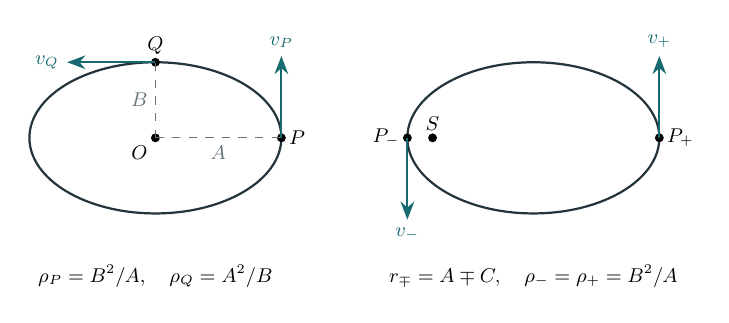
\begin{tikzpicture}[scale=.8,transform shape]

\draw[object] (0,0) ellipse (2 and 1.2);
\fill (0,0) circle (2pt) node[below left] {$O$};
\fill (2,0) circle (2pt) node[right] {$P$};
\fill (0,1.2) circle (2pt) node[above] {$Q$};
\draw[guide] (0,0)--(2,0) node[midway,below] {$A$};
\draw[guide] (0,0)--(0,1.2) node[midway,left] {$B$};
\draw[motion] (2,0)--(2,1.3) node[above] {$v_P$};
\draw[motion] (0,1.2)--(-1.4,1.2) node[left] {$v_Q$};
\node at (0,-2.2) {$\rho_P=B^2/A,\quad\rho_Q=A^2/B$};
\begin{scope}[xshift=6cm]
\draw[object] (0,0) ellipse (2 and 1.2);
\fill (-1.6,0) circle (2pt) node[above] {$S$};
\fill (-2,0) circle (2pt) node[left] {$P_-$};
\fill (2,0) circle (2pt) node[right] {$P_+$};
\draw[motion] (-2,0)--(-2,-1.3) node[below] {$v_-$};
\draw[motion] (2,0)--(2,1.3) node[above] {$v_+$};
\node at (0,-2.2) {$r_\mp=A\mp C,\quad\rho_-=\rho_+=B^2/A$};
\end{scope}

\end{tikzpicture}
\figcaption{解图综一.2A\quad 中心与焦点两种端点比较；力心距离不等同于曲率半径。}
\end{minipage}\end{center}
曲率半径可直接从椭圆参数式推得。令$x=A\cos\phi,y=B\sin\phi$，几何曲率为
\[
\frac1\rho=\frac{|x'y''-y'x''|}{(x'^2+y'^2)^{3/2}}
=\frac{AB}{(A^2\sin^2\phi+B^2\cos^2\phi)^{3/2}}.
\]
在长轴端$\phi=0,\pi$得到$\rho=B^2/A$，短轴端$\phi=\pi/2$得到$\rho=A^2/B$。以中心$O$为力心时，图A中长轴端$P$和短轴端$Q$的切线均垂直于对应的力心半径；以焦点$S$为力心时，选两个长轴端$P_-,P_+$也有这一关系。因此在各自选定的端点，引力完全是法向力，可直接写成$v^2/\rho$。曲线其余位置的法向方向随轨道改变，轴端比较正好避开了切向分量。

解图综一.2A先比较中心力心情形的长轴端$P$和短轴端$Q$。力对中心无力矩，故
\[
Av_P=Bv_Q,\qquad \frac{v_P}{v_Q}=\frac BA.
\]
端点比较中的两个速度由同一守恒量联系。中心力的力矩为零，$m\boldsymbol r\times\boldsymbol v$保持不变；在图A的$P,Q$处，力臂分别为$A,B$，故角动量的大小分别为$mAv_P,mBv_Q$。相除时速度平方比贡献$B^2/A^2$，曲率半径比贡献$A^3/B^3$，最终只剩$A/B$。长短轴不等保证两个不同半径提供独立的幂律信息。

两端速度均垂直于半径，引力完全提供法向加速度：
\[
\frac{GM}{A^\alpha}=\frac{v_P^2}{B^2/A},\qquad
\frac{GM}{B^\alpha}=\frac{v_Q^2}{A^2/B}.
\]
两式相除得
\[
\left(\frac BA\right)^\alpha
=\left(\frac{v_P}{v_Q}\right)^2\frac{A^3}{B^3}
=\frac AB.
\]
因为$A\ne B$，所以$\boxed{\alpha=-1}$。整条椭圆可用参数式表示，取
$x=A\cos nt,y=B\sin nt$，则$\ddot{\boldsymbol r}=-n^2\boldsymbol r$，确为指向中心、大小正比于$r$的力，整条椭圆均满足运动方程。

力心在左焦点$S$时，近日点$P_-$与远日点$P_+$距离分别为$A-C,A+C$，两点曲率半径相同，都是$B^2/A$。角动量守恒给
\[
(A-C)v_-=(A+C)v_+.
\]
两点的法向运动方程相除：
\[
\left(\frac{A+C}{A-C}\right)^\alpha
=\left(\frac{v_-}{v_+}\right)^2
=\left(\frac{A+C}{A-C}\right)^2,
\]
得$\boxed{\alpha=2}$。将运动方程推广到整条轨道，记单位质量角动量$h=r^2\dot\theta$、$u=1/r$，平方反比力的比耐方程为
\[
u''+u=\frac{GM}{h^2}.
\]
比耐方程也可从径向运动逐步导出。以焦点为极点，中心力使$h=r^2\dot\theta$为常量，设$u=1/r$，则
\[
\dot r=-h u',\qquad \ddot r=-h^2u^2u'',\qquad
\ddot r-r\dot\theta^2=-h^2u^2(u''+u).
\]
径向方程右端为$-GM/r^2=-GMu^2$，约去公共因子后得到上述比耐方程。其解中的$p$是半通径，几何关系为$p=B^2/A=A(1-e^2)$，$e=C/A$。在$\theta=0,\pi$时，半径分别为$p/(1+e)=A-C$和$p/(1-e)=A+C$，因而整条极坐标解与题给椭圆的焦点、两轴及端点一致。

其椭圆解$u=(1+e\cos\theta)/p$，其中$p=h^2/(GM)$、$0<e<1$，力心正是焦点。这给出整条椭圆的运动方程。非圆轨道提供两个不同的力心距离；单一圆轨道则给出一个半径处的力。

第（2a）问，以下均取焦点平方反比引力。由近日点的法向方程，
\[
\frac{GM}{(A-C)^2}=\frac{v_-^2}{B^2/A},
\]
得到
\[
\boxed{v_-=\frac B{A-C}\sqrt{\frac{GM}{A}}
=\frac{A+C}{B}\sqrt{\frac{GM}{A}}}.
\]
两种写法由$B^2=(A-C)(A+C)$互换。面积速度恒定，其值可在近日点计算：
\[
\dot{\mathcal A}=\frac12(A-C)v_-=\frac B2\sqrt{\frac{GM}{A}}.
\]
面积速度在任意位置都等于角动量除以$2m$，用近日点是因为该处速度与半径垂直。扫过完整椭圆所需时间等于椭圆面积除以恒定面积速度，所以周期只含半长轴；短半轴既进入面积，也进入面积速度，最终约去。中心力心的线性回复运动则由固定角频率决定周期，同一几何形状在两个力心位置具有不同的时间规律。

椭圆面积为$\pi AB$，故
\[
\boxed{T=\frac{\pi AB}{\dot{\mathcal A}}
=2\pi\sqrt{\frac{A^3}{GM}}}.
\]
\begin{center}\begin{minipage}{.98\linewidth}\centering
\begin{tikzpicture}[scale=.85,transform shape]

\draw[object] (0,0) ellipse (3.8 and .206);
\draw[guide] (-3.8,0)--(3.8,0);
\draw[axis,<->] (-3.8,-1.2)--(3.8,-1.2) node[midway,below] {$2A\simeq4.8\times10^7\,\mathrm{km}$};
\draw[axis,<->] (.7,-.206)--(.7,.206);
\node[above right] at (.7,.206) {$2B\simeq2.6\times10^6\,\mathrm{km}$};
\fill (-3.7944,0) circle (2pt);
\node[above left] at (-3.8,0) {近木端};
\node[above right] at (3.8,0) {远木端};
\node at (0,1.7) {从远木端到近木端约$T/2=380\,\mathrm d$};
\draw[axis,<->] (-3,-3)--(1.75,-3);
\foreach \x/\s in {-3/0,-1.4167/10,.1667/20,1.75/30}{\draw (\x,-2.85)--(\x,-3.15) node[below] {$\s$};}
\node[right] at (2,-3) {$10^6\,\mathrm{km}$};

\end{tikzpicture}
\figcaption{解图综一.2B\quad 读图半轴和时间；轨道长短轴按同一比例绘制。}
\end{minipage}\end{center}
解图综一.2B将轨道长短轴和比例尺放在一起。按题给测量精度，
\[
2A\simeq\frac{5.6}{3.5}(3.0\times10^7)
=4.8\times10^7\,\mathrm{km},
\]
\[
2B\simeq\frac{0.30}{3.5}(3.0\times10^7)
\simeq2.6\times10^6\,\mathrm{km}.
\]
图B的纸面尺寸先由同一标尺换算，再除以2得到半轴。远木端到近木端对应椭圆的一半；两端虽有极大速度差，扫过的面积仍各占半个椭圆，因此所需时间也是半周期。日期间隔按题设粗取$380$天，整周期为$760$天。求引力参数时统一换成米和秒，速度最后再换成千米每秒。短轴的纸面测量仅约$0.30$厘米，读图误差对近点位置和形式近点速度都有明显影响，估算结果用两位有效数字表达。

因此取$A=2.4\times10^7\,\mathrm{km}$、$B=1.3\times10^6\,\mathrm{km}$。从远木端到近木端约半个周期，
$T\simeq760\,\mathrm d=6.57\times10^7\,\mathrm s$。
用周期式消去$GM$，不必另查木星质量：
\[
\sqrt{\frac{GM}{A}}=\frac{2\pi A}{T},\qquad
v_-=\frac{2\pi A(A+C)}{BT}.
\]
轨道很扁，$C\simeq A$，于是
\[
\boxed{v_-\simeq\frac{4\pi A^2}{BT}
\simeq8.5\times10^1\,\mathrm{km/s}}.
\]
该值是把木星作为点引力力心、沿形式椭圆一直走到近木点时的速度。大气入口与形式近点的位置由以下半径比较确定：
\[
r_-=A-C=\frac{B^2}{A+C}\simeq3.52\times10^4\,\mathrm{km}
<r_{\rm atm}.
\]
彗星先穿过大气入口圆，再到达形式近木点；$85\,\mathrm{km/s}$对应形式近点，入口速度在入口半径处计算。
\begin{center}\begin{minipage}{.98\linewidth}\centering
\begin{tikzpicture}[scale=.85,transform shape]
\draw[object] (0,0) circle (1.5);
\draw[traj] plot coordinates {(1.7887149,2.7419037) (1.7685073,2.7309724) (1.7483805,2.7200408) (1.7283344,2.7091086) (1.7083690,2.6981761) (1.6884844,2.6872431) (1.6686805,2.6763097) (1.6489574,2.6653758) (1.6293150,2.6544416) (1.6097533,2.6435069) (1.5902724,2.6325717) (1.5708723,2.6216362) (1.5515529,2.6107002) (1.5323142,2.5997639) (1.5131564,2.5888271) (1.4940793,2.5778899) (1.4750829,2.5669522) (1.4561673,2.5560142) (1.4373325,2.5450758) (1.4185785,2.5341369) (1.3999053,2.5231977) (1.3813128,2.5122580) (1.3628012,2.5013179) (1.3443703,2.4903775) (1.3260202,2.4794366) (1.3077509,2.4684954) (1.2895624,2.4575537) (1.2714548,2.4466117) (1.2534279,2.4356692) (1.2354818,2.4247264) (1.2176165,2.4137832) (1.1998321,2.4028396) (1.1821284,2.3918956) (1.1645056,2.3809513) (1.1469636,2.3700065) (1.1295024,2.3590614) (1.1121221,2.3481159) (1.0948226,2.3371700) (1.0776039,2.3262237) (1.0604660,2.3152771) (1.0434090,2.3043301) (1.0264329,2.2933828) (1.0095375,2.2824350) (0.9927231,2.2714869) (0.9759894,2.2605385) (0.9593366,2.2495897) (0.9427647,2.2386405) (0.9262736,2.2276909) (0.9098634,2.2167410) (0.8935341,2.2057908) (0.8772856,2.1948402) (0.8611180,2.1838892) (0.8450312,2.1729379) (0.8290254,2.1619863) (0.8131004,2.1510343) (0.7972562,2.1400819) (0.7814930,2.1291293) (0.7658106,2.1181762) (0.7502092,2.1072229) (0.7346886,2.0962692) (0.7192489,2.0853151) (0.7038901,2.0743608) (0.6886122,2.0634061) (0.6734152,2.0524510) (0.6582991,2.0414957) (0.6432638,2.0305400) (0.6283095,2.0195840) (0.6134361,2.0086276) (0.5986437,1.9976710) (0.5839321,1.9867140) (0.5693014,1.9757567) (0.5547517,1.9647991) (0.5402829,1.9538412) (0.5258949,1.9428829) (0.5115880,1.9319244) (0.4973619,1.9209655) (0.4832168,1.9100064) (0.4691526,1.8990469) (0.4551693,1.8880871) (0.4412670,1.8771270) (0.4274456,1.8661667) (0.4137051,1.8552060) (0.4000456,1.8442450) (0.3864671,1.8332838) (0.3729694,1.8223222) (0.3595528,1.8113603) (0.3462170,1.8003982) (0.3329623,1.7894358) (0.3197885,1.7784731) (0.3066956,1.7675101) (0.2936837,1.7565468) (0.2807528,1.7455832) (0.2679028,1.7346194) (0.2551338,1.7236552) (0.2424457,1.7126908) (0.2298386,1.7017262) (0.2173125,1.6907612) (0.2048674,1.6797960) (0.1925032,1.6688305) (0.1802201,1.6578648) (0.1680178,1.6468988) (0.1558966,1.6359325) (0.1438564,1.6249660) (0.1318971,1.6139992) (0.1200189,1.6030321) (0.1082216,1.5920648) (0.0965053,1.5810972) (0.0848700,1.5701294) (0.0733157,1.5591613) (0.0618424,1.5481930) (0.0504501,1.5372244) (0.0391388,1.5262556) (0.0279084,1.5152865) (0.0167591,1.5043172) (0.0056908,1.4933477) (-0.0052965,1.4823779) (-0.0162027,1.4714079) (-0.0270280,1.4604376) (-0.0377723,1.4494671) (-0.0484355,1.4384964) (-0.0590178,1.4275255) (-0.0695190,1.4165543) (-0.0799392,1.4055829) (-0.0902784,1.3946113) (-0.1005365,1.3836394) (-0.1107137,1.3726673) (-0.1208098,1.3616950) (-0.1308248,1.3507225) (-0.1407589,1.3397498) (-0.1506119,1.3287768) (-0.1603839,1.3178037) (-0.1700749,1.3068303) (-0.1796848,1.2958567) (-0.1892137,1.2848830) (-0.1986615,1.2739090) (-0.2080283,1.2629348) (-0.2173141,1.2519604) (-0.2265188,1.2409858) (-0.2356425,1.2300110) (-0.2446851,1.2190360) (-0.2536467,1.2080608) (-0.2625273,1.1970854) (-0.2713267,1.1861099) (-0.2800452,1.1751341) (-0.2886826,1.1641582) (-0.2972389,1.1531820) (-0.3057142,1.1422057) (-0.3141084,1.1312292) (-0.3224216,1.1202525) (-0.3306537,1.1092757) (-0.3388047,1.0982986) (-0.3468747,1.0873214) (-0.3548636,1.0763440) (-0.3627715,1.0653664) (-0.3705983,1.0543887) (-0.3783440,1.0434108) (-0.3860086,1.0324327) (-0.3935922,1.0214545) (-0.4010947,1.0104761) (-0.4085162,0.9994976) (-0.4158565,0.9885188) (-0.4231158,0.9775400) (-0.4302941,0.9665609) (-0.4373912,0.9555817) (-0.4444073,0.9446024) (-0.4513422,0.9336229) (-0.4581962,0.9226433) (-0.4649690,0.9116635) (-0.4716607,0.9006836) (-0.4782714,0.8897035) (-0.4848010,0.8787233) (-0.4912494,0.8677429) (-0.4976169,0.8567624) (-0.5039032,0.8457818) (-0.5101084,0.8348010) (-0.5162325,0.8238201) (-0.5222756,0.8128390) (-0.5282375,0.8018579) (-0.5341184,0.7908766) (-0.5399182,0.7798952) (-0.5456369,0.7689136) (-0.5512744,0.7579319) (-0.5568309,0.7469501) (-0.5623063,0.7359682) (-0.5677006,0.7249862) (-0.5730138,0.7140041) (-0.5782459,0.7030218) (-0.5833969,0.6920394) (-0.5884668,0.6810569) (-0.5934556,0.6700744) (-0.5983633,0.6590917) (-0.6031899,0.6481088) (-0.6079353,0.6371259) (-0.6125997,0.6261429) (-0.6171830,0.6151598) (-0.6216852,0.6041766) (-0.6261062,0.5931933) (-0.6304462,0.5822099) (-0.6347050,0.5712264) (-0.6388827,0.5602428) (-0.6429794,0.5492592) (-0.6469949,0.5382754) (-0.6509293,0.5272915) (-0.6547826,0.5163076) (-0.6585547,0.5053236) (-0.6622458,0.4943395) (-0.6658558,0.4833553) (-0.6693846,0.4723711) (-0.6728323,0.4613867) (-0.6761989,0.4504023) (-0.6794844,0.4394179) (-0.6826888,0.4284333) (-0.6858120,0.4174487) (-0.6888542,0.4064640) (-0.6918152,0.3954793) (-0.6946951,0.3844945) (-0.6974939,0.3735096) (-0.7002116,0.3625247) (-0.7028481,0.3515397) (-0.7054035,0.3405547) (-0.7078778,0.3295696) (-0.7102710,0.3185844) (-0.7125831,0.3075992) (-0.7148140,0.2966140) (-0.7169638,0.2856287) (-0.7190325,0.2746433) (-0.7210201,0.2636579) (-0.7229266,0.2526725) (-0.7247519,0.2416870) (-0.7264961,0.2307015) (-0.7281592,0.2197160) (-0.7297411,0.2087304) (-0.7312420,0.1977448) (-0.7326617,0.1867591) (-0.7340003,0.1757734) (-0.7352577,0.1647877) (-0.7364340,0.1538020) (-0.7375292,0.1428163) (-0.7385433,0.1318305) (-0.7394763,0.1208447) (-0.7403281,0.1098589) (-0.7410988,0.0988730) (-0.7417884,0.0878872) (-0.7423968,0.0769013) (-0.7429242,0.0659154) (-0.7433704,0.0549295) (-0.7437354,0.0439436) (-0.7440194,0.0329577) (-0.7442222,0.0219718) (-0.7443439,0.0109859) (-0.7443844,0.0000000) (-0.7443439,-0.0109859) (-0.7442222,-0.0219718) (-0.7440194,-0.0329577) (-0.7437354,-0.0439436) (-0.7433704,-0.0549295) (-0.7429242,-0.0659154) (-0.7423968,-0.0769013) (-0.7417884,-0.0878872) (-0.7410988,-0.0988730) (-0.7403281,-0.1098589) (-0.7394763,-0.1208447) (-0.7385433,-0.1318305) (-0.7375292,-0.1428163) (-0.7364340,-0.1538020) (-0.7352577,-0.1647877) (-0.7340003,-0.1757734) (-0.7326617,-0.1867591) (-0.7312420,-0.1977448) (-0.7297411,-0.2087304) (-0.7281592,-0.2197160) (-0.7264961,-0.2307015) (-0.7247519,-0.2416870) (-0.7229266,-0.2526725) (-0.7210201,-0.2636579) (-0.7190325,-0.2746433) (-0.7169638,-0.2856287) (-0.7148140,-0.2966140) (-0.7125831,-0.3075992) (-0.7102710,-0.3185844) (-0.7078778,-0.3295696) (-0.7054035,-0.3405547) (-0.7028481,-0.3515397) (-0.7002116,-0.3625247) (-0.6974939,-0.3735096) (-0.6946951,-0.3844945) (-0.6918152,-0.3954793) (-0.6888542,-0.4064640) (-0.6858120,-0.4174487) (-0.6826888,-0.4284333) (-0.6794844,-0.4394179) (-0.6761989,-0.4504023) (-0.6728323,-0.4613867) (-0.6693846,-0.4723711) (-0.6658558,-0.4833553) (-0.6622458,-0.4943395) (-0.6585547,-0.5053236) (-0.6547826,-0.5163076) (-0.6509293,-0.5272915) (-0.6469949,-0.5382754) (-0.6429794,-0.5492592) (-0.6388827,-0.5602428) (-0.6347050,-0.5712264) (-0.6304462,-0.5822099) (-0.6261062,-0.5931933) (-0.6216852,-0.6041766) (-0.6171830,-0.6151598) (-0.6125997,-0.6261429) (-0.6079353,-0.6371259) (-0.6031899,-0.6481088) (-0.5983633,-0.6590917) (-0.5934556,-0.6700744) (-0.5884668,-0.6810569) (-0.5833969,-0.6920394) (-0.5782459,-0.7030218) (-0.5730138,-0.7140041) (-0.5677006,-0.7249862) (-0.5623063,-0.7359682) (-0.5568309,-0.7469501) (-0.5512744,-0.7579319) (-0.5456369,-0.7689136) (-0.5399182,-0.7798952) (-0.5341184,-0.7908766) (-0.5282375,-0.8018579) (-0.5222756,-0.8128390) (-0.5162325,-0.8238201) (-0.5101084,-0.8348010) (-0.5039032,-0.8457818) (-0.4976169,-0.8567624) (-0.4912494,-0.8677429) (-0.4848010,-0.8787233) (-0.4782714,-0.8897035) (-0.4716607,-0.9006836) (-0.4649690,-0.9116635) (-0.4581962,-0.9226433) (-0.4513422,-0.9336229) (-0.4444073,-0.9446024) (-0.4373912,-0.9555817) (-0.4302941,-0.9665609) (-0.4231158,-0.9775400) (-0.4158565,-0.9885188) (-0.4085162,-0.9994976) (-0.4010947,-1.0104761) (-0.3935922,-1.0214545) (-0.3860086,-1.0324327) (-0.3783440,-1.0434108) (-0.3705983,-1.0543887) (-0.3627715,-1.0653664) (-0.3548636,-1.0763440) (-0.3468747,-1.0873214) (-0.3388047,-1.0982986) (-0.3306537,-1.1092757) (-0.3224216,-1.1202525) (-0.3141084,-1.1312292) (-0.3057142,-1.1422057) (-0.2972389,-1.1531820) (-0.2886826,-1.1641582) (-0.2800452,-1.1751341) (-0.2713267,-1.1861099) (-0.2625273,-1.1970854) (-0.2536467,-1.2080608) (-0.2446851,-1.2190360) (-0.2356425,-1.2300110) (-0.2265188,-1.2409858) (-0.2173141,-1.2519604) (-0.2080283,-1.2629348) (-0.1986615,-1.2739090) (-0.1892137,-1.2848830) (-0.1796848,-1.2958567) (-0.1700749,-1.3068303) (-0.1603839,-1.3178037) (-0.1506119,-1.3287768) (-0.1407589,-1.3397498) (-0.1308248,-1.3507225) (-0.1208098,-1.3616950) (-0.1107137,-1.3726673) (-0.1005365,-1.3836394) (-0.0902784,-1.3946113) (-0.0799392,-1.4055829) (-0.0695190,-1.4165543) (-0.0590178,-1.4275255) (-0.0484355,-1.4384964) (-0.0377723,-1.4494671) (-0.0270280,-1.4604376) (-0.0162027,-1.4714079) (-0.0052965,-1.4823779) (0.0056908,-1.4933477) (0.0167591,-1.5043172) (0.0279084,-1.5152865) (0.0391388,-1.5262556) (0.0504501,-1.5372244) (0.0618424,-1.5481930) (0.0733157,-1.5591613) (0.0848700,-1.5701294) (0.0965053,-1.5810972) (0.1082216,-1.5920648) (0.1200189,-1.6030321) (0.1318971,-1.6139992) (0.1438564,-1.6249660) (0.1558966,-1.6359325) (0.1680178,-1.6468988) (0.1802201,-1.6578648) (0.1925032,-1.6688305) (0.2048674,-1.6797960) (0.2173125,-1.6907612) (0.2298386,-1.7017262) (0.2424457,-1.7126908) (0.2551338,-1.7236552) (0.2679028,-1.7346194) (0.2807528,-1.7455832) (0.2936837,-1.7565468) (0.3066956,-1.7675101) (0.3197885,-1.7784731) (0.3329623,-1.7894358) (0.3462170,-1.8003982) (0.3595528,-1.8113603) (0.3729694,-1.8223222) (0.3864671,-1.8332838) (0.4000456,-1.8442450) (0.4137051,-1.8552060) (0.4274456,-1.8661667) (0.4412670,-1.8771270) (0.4551693,-1.8880871) (0.4691526,-1.8990469) (0.4832168,-1.9100064) (0.4973619,-1.9209655) (0.5115880,-1.9319244) (0.5258949,-1.9428829) (0.5402829,-1.9538412) (0.5547517,-1.9647991) (0.5693014,-1.9757567) (0.5839321,-1.9867140) (0.5986437,-1.9976710) (0.6134361,-2.0086276) (0.6283095,-2.0195840) (0.6432638,-2.0305400) (0.6582991,-2.0414957) (0.6734152,-2.0524510) (0.6886122,-2.0634061) (0.7038901,-2.0743608) (0.7192489,-2.0853151) (0.7346886,-2.0962692) (0.7502092,-2.1072229) (0.7658106,-2.1181762) (0.7814930,-2.1291293) (0.7972562,-2.1400819) (0.8131004,-2.1510343) (0.8290254,-2.1619863) (0.8450312,-2.1729379) (0.8611180,-2.1838892) (0.8772856,-2.1948402) (0.8935341,-2.2057908) (0.9098634,-2.2167410) (0.9262736,-2.2276909) (0.9427647,-2.2386405) (0.9593366,-2.2495897) (0.9759894,-2.2605385) (0.9927231,-2.2714869) (1.0095375,-2.2824350) (1.0264329,-2.2933828) (1.0434090,-2.3043301) (1.0604660,-2.3152771) (1.0776039,-2.3262237) (1.0948226,-2.3371700) (1.1121221,-2.3481159) (1.1295024,-2.3590614) (1.1469636,-2.3700065) (1.1645056,-2.3809513) (1.1821284,-2.3918956) (1.1998321,-2.4028396) (1.2176165,-2.4137832) (1.2354818,-2.4247264) (1.2534279,-2.4356692) (1.2714548,-2.4466117) (1.2895624,-2.4575537) (1.3077509,-2.4684954) (1.3260202,-2.4794366) (1.3443703,-2.4903775) (1.3628012,-2.5013179) (1.3813128,-2.5122580) (1.3999053,-2.5231977) (1.4185785,-2.5341369) (1.4373325,-2.5450758) (1.4561673,-2.5560142) (1.4750829,-2.5669522) (1.4940793,-2.5778899) (1.5131564,-2.5888271) (1.5323142,-2.5997639) (1.5515529,-2.6107002) (1.5708723,-2.6216362) (1.5902724,-2.6325717) (1.6097533,-2.6435069) (1.6293150,-2.6544416) (1.6489574,-2.6653758) (1.6686805,-2.6763097) (1.6884844,-2.6872431) (1.7083690,-2.6981761) (1.7283344,-2.7091086) (1.7483805,-2.7200408) (1.7685073,-2.7309724) (1.7887149,-2.7419037)};
\fill (0,0) circle (1.8pt) node[below right] {$S$};
\fill (-0.7443844,0) circle (1.8pt) node[below left] {$P_-$};
\fill (0.0123421,1.4999492) circle (2pt) node[above right] {$J$};
\draw[guide] (0,0)--(0.0123421,1.4999492) node[midway,right] {$r_{\rm atm}$};
\node[align=left,right] at (3,0) {圆心$S$为木星中心\\圆周为大气入口\\实线为同一椭圆的局部\\$P_-$位于圆内};
\end{tikzpicture}
\figcaption{解图综一.2C\quad 入口圆与椭圆的真实交点；横纵采用相同长度比例}
\end{minipage}\end{center}
解图综一.2C中的实线由同一个椭圆方程取点绘成，木星中心为焦点$S$，入口圆半径为$r_{\rm atm}$。曲线在$J$第一次穿过入口圆，形式近点$P_-$位于圆内。入口以后的真实运动还受到大气作用；本题把真空椭圆速度计算到$J$，由该处半径代入机械能式。这样近点速度与入口速度各有明确的几何位置。

解图综一.2C放大木星附近的入口$J$，从机械能守恒求入口处速度。把已求得的近日点速度代入单位质量机械能：
\[
\begin{aligned}
\mathcal E&=\frac{v_-^2}{2}-\frac{GM}{A-C}\\
&=\frac{GM}{A-C}\left(\frac{A+C}{2A}-1\right)
=-\frac{GM}{2A}.
\end{aligned}
\]
所以任一点满足
\[
\frac{v^2}{2}-\frac{GM}{r}=-\frac{GM}{2A},
\qquad v^2=GM\left(\frac2r-\frac1A\right).
\]
同一机械能沿整条真空椭圆保持不变。由周期反算
\[
GM=\frac{4\pi^2A^3}{T^2}
\simeq1.27\times10^{17}\,\mathrm{m^3/s^2},
\]
在$r=r_{\rm atm}=7.1\times10^7\,\mathrm m$处，
\[
\boxed{v_{\rm atm}
=\sqrt{\frac{4\pi^2A^3}{T^2}
\left(\frac2{r_{\rm atm}}-\frac1A\right)}
\simeq6.0\times10^1\,\mathrm{km/s}}.
\]
两项速度对应不同位置。图上轴长、时间和忽略扰动的精度共同决定估算精度，结果保留约两位有效数字。
\begin{center}\begin{minipage}{.98\linewidth}\centering
\begin{tikzpicture}[scale=.88,transform shape]
\draw[axis] (0,0.0000000)--(7.25,0.0000000) node[right] {$r/r_{\rm atm}$};
\draw[axis] (0.0000000,0)--(0.0000000,2.8);
\node[above left] at (0.0000000,2.8) {$v/\sqrt{GM/r_{\rm atm}}$};
\node[below,font=\scriptsize] at (0.0000000,-0.0800000) {$1$};
\node[below,font=\scriptsize] at (1.7500000,-0.0800000) {$1.5$};
\node[below,font=\scriptsize] at (3.5000000,-0.0800000) {$2$};
\node[below,font=\scriptsize] at (5.2500000,-0.0800000) {$2.5$};
\node[below,font=\scriptsize] at (7.0000000,-0.0800000) {$3$};
\node[left,font=\scriptsize] at (-0.0800000,0.0000000) {$0$};
\node[left,font=\scriptsize] at (-0.0800000,0.8333333) {$0.5$};
\node[left,font=\scriptsize] at (-0.0800000,1.6666667) {$1$};
\node[left,font=\scriptsize] at (-0.0800000,2.5000000) {$1.5$};
\draw[thick,color=accent] plot coordinates {(0.0000000,2.3552787) (0.0291667,2.3455115) (0.0583333,2.3358646) (0.0875000,2.3263354) (0.1166667,2.3169218) (0.1458333,2.3076212) (0.1750000,2.2984316) (0.2041667,2.2893506) (0.2333333,2.2803762) (0.2625000,2.2715063) (0.2916667,2.2627389) (0.3208333,2.2540721) (0.3500000,2.2455038) (0.3791667,2.2370324) (0.4083333,2.2286558) (0.4375000,2.2203725) (0.4666667,2.2121806) (0.4958333,2.2040786) (0.5250000,2.1960647) (0.5541667,2.1881374) (0.5833333,2.1802952) (0.6125000,2.1725365) (0.6416667,2.1648598) (0.6708333,2.1572638) (0.7000000,2.1497470) (0.7291667,2.1423080) (0.7583333,2.1349455) (0.7875000,2.1276583) (0.8166667,2.1204450) (0.8458333,2.1133044) (0.8750000,2.1062352) (0.9041667,2.0992364) (0.9333333,2.0923067) (0.9625000,2.0854450) (0.9916667,2.0786502) (1.0208333,2.0719213) (1.0500000,2.0652570) (1.0791667,2.0586566) (1.1083333,2.0521188) (1.1375000,2.0456428) (1.1666667,2.0392276) (1.1958333,2.0328721) (1.2250000,2.0265756) (1.2541667,2.0203371) (1.2833333,2.0141557) (1.3125000,2.0080305) (1.3416667,2.0019607) (1.3708333,1.9959455) (1.4000000,1.9899840) (1.4291667,1.9840755) (1.4583333,1.9782192) (1.4875000,1.9724142) (1.5166667,1.9666600) (1.5458333,1.9609556) (1.5750000,1.9553005) (1.6041667,1.9496939) (1.6333333,1.9441351) (1.6625000,1.9386234) (1.6916667,1.9331582) (1.7208333,1.9277389) (1.7500000,1.9223647) (1.7791667,1.9170351) (1.8083333,1.9117495) (1.8375000,1.9065072) (1.8666667,1.9013077) (1.8958333,1.8961503) (1.9250000,1.8910346) (1.9541667,1.8859599) (1.9833333,1.8809258) (2.0125000,1.8759316) (2.0416667,1.8709768) (2.0708333,1.8660610) (2.1000000,1.8611837) (2.1291667,1.8563442) (2.1583333,1.8515422) (2.1875000,1.8467771) (2.2166667,1.8420486) (2.2458333,1.8373560) (2.2750000,1.8326990) (2.3041667,1.8280772) (2.3333333,1.8234900) (2.3625000,1.8189371) (2.3916667,1.8144179) (2.4208333,1.8099322) (2.4500000,1.8054795) (2.4791667,1.8010594) (2.5083333,1.7966715) (2.5375000,1.7923154) (2.5666667,1.7879907) (2.5958333,1.7836970) (2.6250000,1.7794341) (2.6541667,1.7752014) (2.6833333,1.7709987) (2.7125000,1.7668256) (2.7416667,1.7626818) (2.7708333,1.7585669) (2.8000000,1.7544806) (2.8291667,1.7504225) (2.8583333,1.7463924) (2.8875000,1.7423899) (2.9166667,1.7384146) (2.9458333,1.7344664) (2.9750000,1.7305448) (3.0041667,1.7266497) (3.0333333,1.7227806) (3.0625000,1.7189373) (3.0916667,1.7151195) (3.1208333,1.7113270) (3.1500000,1.7075594) (3.1791667,1.7038165) (3.2083333,1.7000980) (3.2375000,1.6964036) (3.2666667,1.6927332) (3.2958333,1.6890864) (3.3250000,1.6854629) (3.3541667,1.6818626) (3.3833333,1.6782852) (3.4125000,1.6747304) (3.4416667,1.6711980) (3.4708333,1.6676878) (3.5000000,1.6641996) (3.5291667,1.6607330) (3.5583333,1.6572879) (3.5875000,1.6538642) (3.6166667,1.6504614) (3.6458333,1.6470795) (3.6750000,1.6437182) (3.7041667,1.6403773) (3.7333333,1.6370566) (3.7625000,1.6337560) (3.7916667,1.6304751) (3.8208333,1.6272138) (3.8500000,1.6239720) (3.8791667,1.6207494) (3.9083333,1.6175458) (3.9375000,1.6143610) (3.9666667,1.6111949) (3.9958333,1.6080473) (4.0250000,1.6049180) (4.0541667,1.6018068) (4.0833333,1.5987135) (4.1125000,1.5956381) (4.1416667,1.5925802) (4.1708333,1.5895398) (4.2000000,1.5865166) (4.2291667,1.5835106) (4.2583333,1.5805215) (4.2875000,1.5775491) (4.3166667,1.5745935) (4.3458333,1.5716543) (4.3750000,1.5687314) (4.4041667,1.5658247) (4.4333333,1.5629340) (4.4625000,1.5600592) (4.4916667,1.5572002) (4.5208333,1.5543567) (4.5500000,1.5515287) (4.5791667,1.5487160) (4.6083333,1.5459185) (4.6375000,1.5431360) (4.6666667,1.5403684) (4.6958333,1.5376156) (4.7250000,1.5348774) (4.7541667,1.5321537) (4.7833333,1.5294444) (4.8125000,1.5267494) (4.8416667,1.5240685) (4.8708333,1.5214016) (4.9000000,1.5187486) (4.9291667,1.5161093) (4.9583333,1.5134837) (4.9875000,1.5108717) (5.0166667,1.5082730) (5.0458333,1.5056876) (5.0750000,1.5031155) (5.1041667,1.5005564) (5.1333333,1.4980102) (5.1625000,1.4954770) (5.1916667,1.4929564) (5.2208333,1.4904485) (5.2500000,1.4879532) (5.2791667,1.4854702) (5.3083333,1.4829996) (5.3375000,1.4805413) (5.3666667,1.4780950) (5.3958333,1.4756608) (5.4250000,1.4732385) (5.4541667,1.4708280) (5.4833333,1.4684293) (5.5125000,1.4660422) (5.5416667,1.4636666) (5.5708333,1.4613025) (5.6000000,1.4589498) (5.6291667,1.4566083) (5.6583333,1.4542781) (5.6875000,1.4519589) (5.7166667,1.4496507) (5.7458333,1.4473534) (5.7750000,1.4450669) (5.8041667,1.4427912) (5.8333333,1.4405262) (5.8625000,1.4382717) (5.8916667,1.4360278) (5.9208333,1.4337942) (5.9500000,1.4315710) (5.9791667,1.4293581) (6.0083333,1.4271553) (6.0375000,1.4249626) (6.0666667,1.4227799) (6.0958333,1.4206072) (6.1250000,1.4184444) (6.1541667,1.4162913) (6.1833333,1.4141480) (6.2125000,1.4120143) (6.2416667,1.4098902) (6.2708333,1.4077756) (6.3000000,1.4056704) (6.3291667,1.4035746) (6.3583333,1.4014881) (6.3875000,1.3994109) (6.4166667,1.3973427) (6.4458333,1.3952837) (6.4750000,1.3932337) (6.5041667,1.3911927) (6.5333333,1.3891605) (6.5625000,1.3871372) (6.5916667,1.3851226) (6.6208333,1.3831168) (6.6500000,1.3811196) (6.6791667,1.3791309) (6.7083333,1.3771508) (6.7375000,1.3751791) (6.7666667,1.3732159) (6.7958333,1.3712609) (6.8250000,1.3693143) (6.8541667,1.3673758) (6.8833333,1.3654456) (6.9125000,1.3635234) (6.9416667,1.3616093) (6.9708333,1.3597031) (7.0000000,1.3578049)};
\end{tikzpicture}
\figcaption{解图综一.2D\quad 同一真空椭圆上不同半径对应的速度}
\end{minipage}\end{center}
解图综一.2D画$v/\sqrt{GM/r_{\rm atm}}$随$r/r_{\rm atm}$的变化。沿入射支，半径减小，势能降低，速度增加；在入口圆上速度约为$60\ \mathrm{km/s}$。形式近点处约$85\ \mathrm{km/s}$对应更小的半径。若形式近点恰好接近所取入口圆，两数才会接近；本题的两半径相差约一倍，分开代入机械能式可以保留这一几何差异。



\Needspace{13\baselineskip}

\pdfbookmark[2]{第 3 题 四维理想气体的统计规律和热过程}{q3}

\section*{第 3 题\quad 四维理想气体的统计规律和热过程}\label{q:3}


设想四维欧氏空间中的单原子理想气体，分子质量为$m$，温度为$T$，四个直角坐标方向等价且相互独立。气体占有的四维体积记为$V_4$，分子数$N$，物质的量$\nu=N/N_A$，$R=N_Ak_B$。
\begin{enumerate}
\item 分别求：（a）方均根速率；（b）四维速度矢量的归一化概率密度$F_4(v_1,v_2,v_3,v_4)$；（c）速率概率密度$f_4(v)$；（d）平均速率。推导四维速度壳的几何因子。
\item 四维压强定义为单位三维超面积上的法向力，气体做功仍记作$p\,dV_4$。求：（a）状态方程；（b）绝热过程$p$与$V_4$关系；（c）在$p$正比于$V_4$的直线过程中，摩尔热容$C$。结果用$R$表示，并写出一般常热容多方过程关系。
\end{enumerate}


\begin{center}\begin{minipage}{.98\linewidth}\centering
\begin{tikzpicture}[scale=.8,transform shape]

\draw[axis] (0,0)--(3.4,0) node[right] {$v_1$};
\draw[axis] (0,0)--(0,2.5) node[above] {$v_2$};
\draw[axis] (0,0)--(-1.8,-1.4) node[below left] {$v_3$};
\draw[axis] (0,0)--(1.8,-1.5) node[below right] {$v_4$};
\node[align=left] at (6,1.5) {四个独立分量\\$v^2=\sum_{i=1}^4v_i^2$};
\begin{scope}[xshift=5cm,yshift=-2cm]
\draw[axis] (0,0)--(4,0) node[right] {$V_4$};
\draw[axis] (0,0)--(0,2.5) node[above] {$p$};
\draw[traj] (0,0)--(3.5,2.1) node[right] {$p=aV_4$};
\end{scope}

\end{tikzpicture}
\figcaption{图综一.3\quad 四个速度坐标的符号投影及所求热过程路径。}
\end{minipage}\end{center}

\Needspace{6\baselineskip}\subsection*{解答}


图综一.3用四个坐标方向表示分子速度的四个分量。能量均分给出每一分量的平均动能$k_BT/2$，所以
\[
\frac12m\langle v^2\rangle
=\sum_{i=1}^4\frac12m\langle v_i^2\rangle=2k_BT,
\qquad
\boxed{v_{\rm rms}=2\sqrt{\frac{k_BT}{m}}}.
\]
总平动能$2k_BT$与单分量动能$k_BT/2$分别对应总内能和单向压强，计算时应分开。

从三维到四维，概率相乘的依据是各正交分量独立，分量的分布仍为一维正态分布。四维联合密度描述速度矢量落在一个微小四维长方体内的概率，四个微分速度分量共同构成积分元。只给速率大小时，方向全部保留为同一速率的不同状态，故要把整层速度壳上的概率加起来。接下来的超面积因子正是这一步对方向的求和。

四个分量各服从一维高斯分布，独立性使联合密度为四个因子的乘积：
\[
\begin{aligned}
F_4(\boldsymbol v)
&=\prod_{i=1}^4\sqrt{\frac{m}{2\pi k_BT}}
\exp\left(-\frac{mv_i^2}{2k_BT}\right)\\
&=\boxed{\left(\frac{m}{2\pi k_BT}\right)^2
\exp\left(-\frac{mv^2}{2k_BT}\right)}.
\end{aligned}
\]
其含义是$dP=F_4\,dv_1dv_2dv_3dv_4$，在整个四维速度空间积分为一；速率区间的概率通过整层速度壳积分得到，下面用壳的超面积构造径向密度。
\begin{center}\begin{minipage}{.98\linewidth}\centering
\begin{tikzpicture}[scale=.8,transform shape]

\draw[object] (0,0) circle (2.4);
\draw[axis] (0,-2.8)--(0,3) node[above] {$v_4$方向};
\draw[guide] (0,0)--(2.078,1.2) node[midway,below] {$a$};
\draw[object] (-2.078,1.2)--(2.078,1.2);
\draw[guide] (-2.078,1.2) ellipse (0.02 and .02);
\draw[guide] (0,1.2) ellipse (2.078 and .35);
\draw[axis,<->] (0,1.6)--(2.078,1.6) node[midway,above] {$a\sin\varphi$};
\draw[object] (0,.8) arc[start angle=90,end angle=30,radius=.8];
\node at (.48,.85) {$\varphi$};
\draw[traj] (30:2.4) arc[start angle=30,end angle=20,radius=2.4];
\node[right] at (2.5,.85) {$a\,d\varphi$};
\node[align=left] at (6.3,1) {纬面为二维球面\\面积$4\pi a^2\sin^2\varphi$\\乘子午弧宽$a\,d\varphi$};
\node at (3,-3.7) {纸上仅画子午截面，纬圈表示球面纬带的投影};

\end{tikzpicture}
\figcaption{解图综一.3A\quad 四维球面超面积的纬带积分，子午弧宽与纬面超面积相乘。}
\end{minipage}\end{center}
解图综一.3A画四维球面的一条子午截面，借纬带计算超面积。半径$a$的三维球面超面积记作$S_3(a)$。用第四坐标方向作极轴，极角$\varphi$处的纬面是半径$a\sin\varphi$的普通二维球面，其面积为$4\pi a^2\sin^2\varphi$；沿子午线的厚度是$a\,d\varphi$，所以
\[
\begin{aligned}
S_3(a)&=\int_0^\pi
4\pi a^2\sin^2\varphi\;a\,d\varphi\\
&=4\pi a^3\frac{\pi}{2}
=\boxed{2\pi^2a^3}.
\end{aligned}
\]
以第四轴作极轴，极角从0变到$\pi$时覆盖整个超球面。固定极角后还有三个坐标方向，固定它们的半径$a\sin\varphi$形成普通二维球面；再沿子午线移动$a\,\mathrm d\varphi$，这些球面扫出三维超面积元。第四坐标的投影变化是$-a\sin\varphi\,\mathrm d\varphi$，子午弧长则为$a\,\mathrm d\varphi$，积分元取后者。径向再增加$\mathrm da$，扫出的薄层体积为$S_3(a)\mathrm da$，与后面的速度壳体积完全对应。

纬带宽度沿超球面子午线取弧长$a\,d\varphi$。再径向积分，四维球体积为$V_4(a)=\pi^2a^4/2$，对$a$求导也回到同一个$S_3(a)$。

速率在$v$与$v+dv$之间，对应厚度$dv$的四维速度壳，故
\[
\boxed{f_4(v)=S_3(v)F_4(v)
=\frac{m^2}{2(k_BT)^2}v^3
\exp\left(-\frac{mv^2}{2k_BT}\right)},\qquad v\geq0.
\]
令$b=m/(2k_BT)$，则$f_4(v)=2b^2v^3e^{-bv^2}$。用$x=bv^2$变换，归一化积分为
$\int_0^\infty f_4(v)dv=\int_0^\infty xe^{-x}dx=1$。
\begin{center}\begin{minipage}{.98\linewidth}\centering
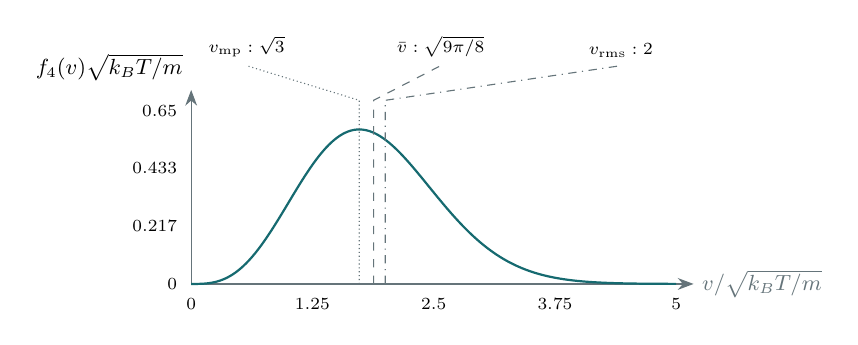
\begin{tikzpicture}[scale=.88,transform shape]
\draw[axis] (0,0.0000000)--(7.25,0.0000000) node[right] {$v/\sqrt{k_BT/m}$};
\draw[axis] (0.0000000,0)--(0.0000000,2.8);
\node[above left] at (0.0000000,2.8) {$f_4(v)\sqrt{k_BT/m}$};
\node[below,font=\scriptsize] at (0.0000000,-0.0800000) {$0$};
\node[below,font=\scriptsize] at (1.7500000,-0.0800000) {$1.25$};
\node[below,font=\scriptsize] at (3.5000000,-0.0800000) {$2.5$};
\node[below,font=\scriptsize] at (5.2500000,-0.0800000) {$3.75$};
\node[below,font=\scriptsize] at (7.0000000,-0.0800000) {$5$};
\node[left,font=\scriptsize] at (-0.0800000,0.0000000) {$0$};
\node[left,font=\scriptsize] at (-0.0800000,0.8333333) {$0.217$};
\node[left,font=\scriptsize] at (-0.0800000,1.6666667) {$0.433$};
\node[left,font=\scriptsize] at (-0.0800000,2.5000000) {$0.65$};
\draw[thick,color=accent] plot coordinates {(0.0000000,0.0000000) (0.0291667,0.0000174) (0.0583333,0.0001390) (0.0875000,0.0004686) (0.1166667,0.0011090) (0.1458333,0.0021619) (0.1750000,0.0037268) (0.2041667,0.0059013) (0.2333333,0.0087803) (0.2625000,0.0124556) (0.2916667,0.0170156) (0.3208333,0.0225448) (0.3500000,0.0291236) (0.3791667,0.0368277) (0.4083333,0.0457282) (0.4375000,0.0558909) (0.4666667,0.0673760) (0.4958333,0.0802384) (0.5250000,0.0945266) (0.5541667,0.1102834) (0.5833333,0.1275451) (0.6125000,0.1463415) (0.6416667,0.1666959) (0.6708333,0.1886250) (0.7000000,0.2121387) (0.7291667,0.2372401) (0.7583333,0.2639255) (0.7875000,0.2921847) (0.8166667,0.3220006) (0.8458333,0.3533495) (0.8750000,0.3862012) (0.9041667,0.4205191) (0.9333333,0.4562606) (0.9625000,0.4933768) (0.9916667,0.5318132) (1.0208333,0.5715094) (1.0500000,0.6123999) (1.0791667,0.6544142) (1.1083333,0.6974767) (1.1375000,0.7415077) (1.1666667,0.7864230) (1.1958333,0.8321349) (1.2250000,0.8785520) (1.2541667,0.9255798) (1.2833333,0.9731213) (1.3125000,1.0210768) (1.3416667,1.0693449) (1.3708333,1.1178225) (1.4000000,1.1664051) (1.4291667,1.2149877) (1.4583333,1.2634647) (1.4875000,1.3117304) (1.5166667,1.3596795) (1.5458333,1.4072074) (1.5750000,1.4542104) (1.6041667,1.5005864) (1.6333333,1.5462350) (1.6625000,1.5910579) (1.6916667,1.6349590) (1.7208333,1.6778453) (1.7500000,1.7196265) (1.7791667,1.7602157) (1.8083333,1.7995294) (1.8375000,1.8374881) (1.8666667,1.8740161) (1.8958333,1.9090420) (1.9250000,1.9424988) (1.9541667,1.9743238) (1.9833333,2.0044593) (2.0125000,2.0328522) (2.0416667,2.0594544) (2.0708333,2.0842228) (2.1000000,2.1071194) (2.1291667,2.1281110) (2.1583333,2.1471699) (2.1875000,2.1642733) (2.2166667,2.1794035) (2.2458333,2.1925480) (2.2750000,2.2036992) (2.3041667,2.2128545) (2.3333333,2.2200161) (2.3625000,2.2251910) (2.3916667,2.2283910) (2.4208333,2.2296321) (2.4500000,2.2289349) (2.4791667,2.2263241) (2.5083333,2.2218287) (2.5375000,2.2154813) (2.5666667,2.2073183) (2.5958333,2.1973795) (2.6250000,2.1857083) (2.6541667,2.1723509) (2.6833333,2.1573565) (2.7125000,2.1407769) (2.7416667,2.1226665) (2.7708333,2.1030817) (2.8000000,2.0820813) (2.8291667,2.0597254) (2.8583333,2.0360761) (2.8875000,2.0111966) (2.9166667,1.9851512) (2.9458333,1.9580054) (2.9750000,1.9298251) (3.0041667,1.9006768) (3.0333333,1.8706275) (3.0625000,1.8397439) (3.0916667,1.8080929) (3.1208333,1.7757412) (3.1500000,1.7427549) (3.1791667,1.7091994) (3.2083333,1.6751396) (3.2375000,1.6406392) (3.2666667,1.6057611) (3.2958333,1.5705668) (3.3250000,1.5351165) (3.3541667,1.4994691) (3.3833333,1.4636819) (3.4125000,1.4278104) (3.4416667,1.3919086) (3.4708333,1.3560285) (3.5000000,1.3202204) (3.5291667,1.2845324) (3.5583333,1.2490108) (3.5875000,1.2136998) (3.6166667,1.1786416) (3.6458333,1.1438762) (3.6750000,1.1094414) (3.7041667,1.0753731) (3.7333333,1.0417049) (3.7625000,1.0084682) (3.7916667,0.9756924) (3.8208333,0.9434047) (3.8500000,0.9116303) (3.8791667,0.8803921) (3.9083333,0.8497114) (3.9375000,0.8196070) (3.9666667,0.7900960) (3.9958333,0.7611937) (4.0250000,0.7329132) (4.0541667,0.7052661) (4.0833333,0.6782621) (4.1125000,0.6519092) (4.1416667,0.6262138) (4.1708333,0.6011807) (4.2000000,0.5768133) (4.2291667,0.5531133) (4.2583333,0.5300814) (4.2875000,0.5077166) (4.3166667,0.4860169) (4.3458333,0.4649790) (4.3750000,0.4445987) (4.4041667,0.4248706) (4.4333333,0.4057882) (4.4625000,0.3873445) (4.4916667,0.3695312) (4.5208333,0.3523396) (4.5500000,0.3357600) (4.5791667,0.3197824) (4.6083333,0.3043959) (4.6375000,0.2895892) (4.6666667,0.2753504) (4.6958333,0.2616675) (4.7250000,0.2485279) (4.7541667,0.2359187) (4.7833333,0.2238268) (4.8125000,0.2122388) (4.8416667,0.2011412) (4.8708333,0.1905205) (4.9000000,0.1803628) (4.9291667,0.1706545) (4.9583333,0.1613817) (4.9875000,0.1525308) (5.0166667,0.1440879) (5.0458333,0.1360394) (5.0750000,0.1283720) (5.1041667,0.1210721) (5.1333333,0.1141266) (5.1625000,0.1075225) (5.1916667,0.1012468) (5.2208333,0.0952871) (5.2500000,0.0896308) (5.2791667,0.0842659) (5.3083333,0.0791806) (5.3375000,0.0743630) (5.3666667,0.0698021) (5.3958333,0.0654866) (5.4250000,0.0614059) (5.4541667,0.0575495) (5.4833333,0.0539073) (5.5125000,0.0504694) (5.5416667,0.0472262) (5.5708333,0.0441687) (5.6000000,0.0412877) (5.6291667,0.0385748) (5.6583333,0.0360216) (5.6875000,0.0336201) (5.7166667,0.0313626) (5.7458333,0.0292418) (5.7750000,0.0272504) (5.8041667,0.0253816) (5.8333333,0.0236290) (5.8625000,0.0219862) (5.8916667,0.0204472) (5.9208333,0.0190063) (5.9500000,0.0176580) (5.9791667,0.0163970) (6.0083333,0.0152184) (6.0375000,0.0141174) (6.0666667,0.0130894) (6.0958333,0.0121302) (6.1250000,0.0112356) (6.1541667,0.0104018) (6.1833333,0.0096250) (6.2125000,0.0089018) (6.2416667,0.0082288) (6.2708333,0.0076029) (6.3000000,0.0070211) (6.3291667,0.0064805) (6.3583333,0.0059787) (6.3875000,0.0055129) (6.4166667,0.0050809) (6.4458333,0.0046804) (6.4750000,0.0043094) (6.5041667,0.0039658) (6.5333333,0.0036478) (6.5625000,0.0033537) (6.5916667,0.0030817) (6.6208333,0.0028304) (6.6500000,0.0025983) (6.6791667,0.0023841) (6.7083333,0.0021865) (6.7375000,0.0020042) (6.7666667,0.0018363) (6.7958333,0.0016816) (6.8250000,0.0015391) (6.8541667,0.0014081) (6.8833333,0.0012876) (6.9125000,0.0011768) (6.9416667,0.0010750) (6.9708333,0.0009816) (7.0000000,0.0008958)};
\draw[guide,densely dotted] (2.4248711,0)--(2.4248711,2.65)--(0.8,3.15);
\node[above,font=\scriptsize] at (0.8,3.15) {$v_{\rm mp}:\sqrt3$};
\draw[guide,dashed] (2.6319597,0)--(2.6319597,2.65)--(3.6,3.15);
\node[above,font=\scriptsize] at (3.6,3.15) {$\bar v:\sqrt{9\pi/8}$};
\draw[guide,dashdotted] (2.8000000,0)--(2.8000000,2.65)--(6.2,3.15);
\node[above,font=\scriptsize] at (6.2,3.15) {$v_{\rm rms}:2$};
\end{tikzpicture}
\figcaption{解图综一.3B\quad 归一化速率分布与三个典型速率}
\end{minipage}\end{center}
解图综一.3B中的分布在$v=0$为零，峰位、平均值和方均根对应三个不同位置。平均速率由
\[
\bar v=2b^2\int_0^\infty v^4e^{-bv^2}dv.
\]
一般积分用$x=bv^2$可得
\[
\int_0^\infty v^k e^{-bv^2}dv
=\frac{\Gamma[(k+1)/2]}{2b^{(k+1)/2}}.
\]
取$k=4$，利用$\Gamma(5/2)=\frac32\frac12\sqrt\pi$，
\[
\boxed{\bar v=\frac{3\sqrt\pi}{4\sqrt b}
=\frac{3\sqrt{2\pi}}4\sqrt{\frac{k_BT}{m}}
=\sqrt{\frac{9\pi k_BT}{8m}}}.
\]
四维平均速率积分中的$v^4e^{-bv^2}$也出现在三维气体的均方速率积分中。若以$f_3$表示同温、同质量的三维速率密度，则
\[
\int_0^\infty v^2f_3(v)\,\mathrm dv
=4\pi\left(\frac{m}{2\pi k_BT}\right)^{3/2}
\int_0^\infty v^4e^{-bv^2}\,\mathrm dv=\frac{3k_BT}{m}.
\]
将同一个积分代回四维平均速率，得到
\[
\bar v=\frac\pi2\left(\frac{m}{2\pi k_BT}\right)^{1/2}
\frac{3k_BT}{m}=\sqrt{\frac{9\pi k_BT}{8m}}.
\]
这说明维数变化后，同一个高斯径向积分会进入不同阶矩。上面的伽马函数方法给出任意阶矩，三维均方值则为这一个积分提供直接的物理解释。

由$f_4$求导还有$v_{\rm mp}=\sqrt{3k_BT/m}$，满足
$v_{\rm mp}<\bar v<v_{\rm rms}$，分别对应速率密度的峰值位置、速率的一阶矩与二阶矩的平方根。

法向为第一坐标方向的壁面只改变碰撞分子的第一速度分量。每次弹性反射传给壁的法向动量为$2m|v_1|$，单位时间内到达单位超面积的分子数又与$|v_1|$成正比。将朝向壁的一半分布相加，因分布关于$v_1=0$对称，得到$2\int_0^\infty mv_1^2F_1(v_1)\,\mathrm dv_1=m\langle v_1^2\rangle$。其他三个分量随其归一化积分约去，因此压强只取一个分量的均方值。

第（2a）问，取与第一坐标轴垂直的一面壁。分子碰壁的法向动量通量只包含$v_1$，同三维情形的碰撞计数给
\[
p=\frac{Nm}{V_4}\langle v_1^2\rangle
=\frac{N}{V_4}k_BT.
\]
于是
\[
\boxed{pV_4=Nk_BT=\nu RT}.
\]
若用$\epsilon_1=m\langle v_1^2\rangle/2$表示单分量平均动能，则$p=2(N/V_4)\epsilon_1$。压强使用单方向动能，内能则累加四个方向。

总内能与摩尔热容为
\[
U=2\nu RT,\qquad C_V=2R,\qquad C_p=C_V+R=3R.
\]
定压摩尔热容也可从第一定律逐项求出。在定压过程中，对$pV_4=\nu RT$微分有$p\,\mathrm dV_4=\nu R\,\mathrm dT$；内能增量为$2\nu R\,\mathrm dT$，两者相加给$\delta Q=3\nu R\,\mathrm dT$，所以$C_p=3R$。在准静态绝热过程中，内能增量$2\nu R\,\mathrm dT$与体积功$p\,\mathrm dV_4$之和为零；对一般路径，两者按该路径的$T,V_4$关系共同决定吸热量。

第（2b）问，准静态绝热过程满足
\[
0=dU+p\,dV_4
=\nu C_VdT+\nu RT\frac{dV_4}{V_4}.
\]
除以$\nu C_VT$并积分：
\[
\frac{dT}{T}+\frac{R}{C_V}\frac{dV_4}{V_4}=0
\ \Longrightarrow\ TV_4^{1/2}=\text{常量},
\]
再消去$T$，
\[
\boxed{pV_4^{3/2}=\text{常量}},\qquad \gamma=\frac32.
\]
\begin{center}\begin{minipage}{.98\linewidth}\centering
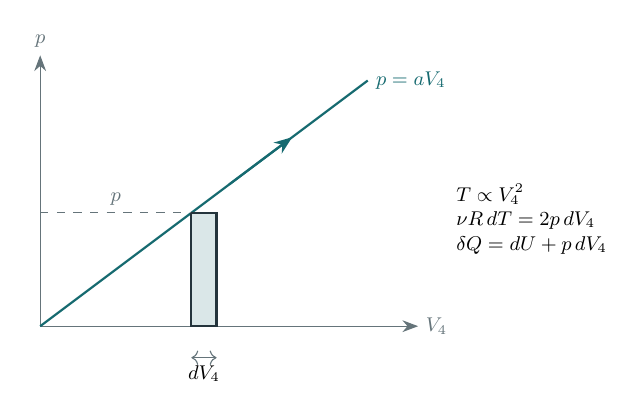
\begin{tikzpicture}[scale=.8,transform shape]

\draw[axis] (0,0)--(6,0) node[right] {$V_4$};
\draw[axis] (0,0)--(0,4.3) node[above] {$p$};
\draw[traj] (0,0)--(5.2,3.9) node[right] {$p=aV_4$};
\fill[accent!16] (2.4,0) rectangle (2.8,1.8);
\draw[object] (2.4,0) rectangle (2.8,1.8);
\draw[axis,<->] (2.4,-.5)--(2.8,-.5);
\node[below] at (2.6,-.5) {$dV_4$};
\draw[guide] (0,1.8)--(2.4,1.8) node[midway,above] {$p$};
\draw[motion] (3,2.25)--(4,3);
\node[align=left] at (7.8,1.7) {$T\propto V_4^2$\\$\nu R\,dT=2p\,dV_4$\\$\delta Q=dU+p\,dV_4$};

\end{tikzpicture}
\figcaption{解图综一.3C\quad 直线路径上的温升与体积功；两项相加求路径热容。}
\end{minipage}\end{center}
第（2c）问，解图综一.3C中的路径通过坐标原点，$p=aV_4$，斜率$a>0$，膨胀时压强随体积增加。由状态方程
\[
T=\frac{aV_4^2}{\nu R},\qquad
\nu R\,dT=2aV_4\,dV_4=2p\,dV_4.
\]
热力学第一定律给
\[
\delta Q=2\nu R\,dT+p\,dV_4
=\left(2+\frac12\right)\nu R\,dT,
\quad
\boxed{C=\frac{\delta Q}{\nu\,dT}=\frac52R}.
\]
沿这条路径膨胀时温度上升、吸热且对外做功。图中曲线下的面积正是$p\,dV_4$；沿路径的温升率把体积功换成每单位温升所需的热量。

对任一常摩尔热容$C$，有
\[
\nu(C-C_V)dT=p\,dV_4,\qquad
(C-C_V)\frac{dT}{T}=R\frac{dV_4}{V_4}.
\]
若$C\ne C_V$，结合$pV_4=\nu RT$，积分得到
\[
\boxed{pV_4^n=\text{常量},\qquad
n=1-\frac{R}{C-C_V}
=\frac{C-C_V-R}{C-C_V}}.
\]
本题$C-C_V=R/2$，所以$n=-1$，确为$p/V_4$恒定。$C=C_V$时由第一条微分关系得到$p\,dV_4=0$，对应等容过程，另用定容关系描述。
\begin{center}\begin{minipage}{.98\linewidth}\centering
\begin{tikzpicture}[scale=.88,transform shape]
\draw[axis] (0,0.0000000)--(7.25,0.0000000) node[right] {$V_4/V_i$};
\draw[axis] (0.0000000,0)--(0.0000000,2.8);
\node[above left] at (0.0000000,2.8) {$p/p_i$};
\node[below,font=\scriptsize] at (0.0000000,-0.0800000) {$0.5$};
\node[below,font=\scriptsize] at (1.7500000,-0.0800000) {$0.875$};
\node[below,font=\scriptsize] at (3.5000000,-0.0800000) {$1.25$};
\node[below,font=\scriptsize] at (5.2500000,-0.0800000) {$1.62$};
\node[below,font=\scriptsize] at (7.0000000,-0.0800000) {$2$};
\node[left,font=\scriptsize] at (-0.0800000,0.0000000) {$0$};
\node[left,font=\scriptsize] at (-0.0800000,0.8333333) {$1$};
\node[left,font=\scriptsize] at (-0.0800000,1.6666667) {$2$};
\node[left,font=\scriptsize] at (-0.0800000,2.5000000) {$3$};
\draw[thick,color=accent] plot coordinates {(0.0000000,0.4166667) (0.0291667,0.4218750) (0.0583333,0.4270833) (0.0875000,0.4322917) (0.1166667,0.4375000) (0.1458333,0.4427083) (0.1750000,0.4479167) (0.2041667,0.4531250) (0.2333333,0.4583333) (0.2625000,0.4635417) (0.2916667,0.4687500) (0.3208333,0.4739583) (0.3500000,0.4791667) (0.3791667,0.4843750) (0.4083333,0.4895833) (0.4375000,0.4947917) (0.4666667,0.5000000) (0.4958333,0.5052083) (0.5250000,0.5104167) (0.5541667,0.5156250) (0.5833333,0.5208333) (0.6125000,0.5260417) (0.6416667,0.5312500) (0.6708333,0.5364583) (0.7000000,0.5416667) (0.7291667,0.5468750) (0.7583333,0.5520833) (0.7875000,0.5572917) (0.8166667,0.5625000) (0.8458333,0.5677083) (0.8750000,0.5729167) (0.9041667,0.5781250) (0.9333333,0.5833333) (0.9625000,0.5885417) (0.9916667,0.5937500) (1.0208333,0.5989583) (1.0500000,0.6041667) (1.0791667,0.6093750) (1.1083333,0.6145833) (1.1375000,0.6197917) (1.1666667,0.6250000) (1.1958333,0.6302083) (1.2250000,0.6354167) (1.2541667,0.6406250) (1.2833333,0.6458333) (1.3125000,0.6510417) (1.3416667,0.6562500) (1.3708333,0.6614583) (1.4000000,0.6666667) (1.4291667,0.6718750) (1.4583333,0.6770833) (1.4875000,0.6822917) (1.5166667,0.6875000) (1.5458333,0.6927083) (1.5750000,0.6979167) (1.6041667,0.7031250) (1.6333333,0.7083333) (1.6625000,0.7135417) (1.6916667,0.7187500) (1.7208333,0.7239583) (1.7500000,0.7291667) (1.7791667,0.7343750) (1.8083333,0.7395833) (1.8375000,0.7447917) (1.8666667,0.7500000) (1.8958333,0.7552083) (1.9250000,0.7604167) (1.9541667,0.7656250) (1.9833333,0.7708333) (2.0125000,0.7760417) (2.0416667,0.7812500) (2.0708333,0.7864583) (2.1000000,0.7916667) (2.1291667,0.7968750) (2.1583333,0.8020833) (2.1875000,0.8072917) (2.2166667,0.8125000) (2.2458333,0.8177083) (2.2750000,0.8229167) (2.3041667,0.8281250) (2.3333333,0.8333333) (2.3625000,0.8385417) (2.3916667,0.8437500) (2.4208333,0.8489583) (2.4500000,0.8541667) (2.4791667,0.8593750) (2.5083333,0.8645833) (2.5375000,0.8697917) (2.5666667,0.8750000) (2.5958333,0.8802083) (2.6250000,0.8854167) (2.6541667,0.8906250) (2.6833333,0.8958333) (2.7125000,0.9010417) (2.7416667,0.9062500) (2.7708333,0.9114583) (2.8000000,0.9166667) (2.8291667,0.9218750) (2.8583333,0.9270833) (2.8875000,0.9322917) (2.9166667,0.9375000) (2.9458333,0.9427083) (2.9750000,0.9479167) (3.0041667,0.9531250) (3.0333333,0.9583333) (3.0625000,0.9635417) (3.0916667,0.9687500) (3.1208333,0.9739583) (3.1500000,0.9791667) (3.1791667,0.9843750) (3.2083333,0.9895833) (3.2375000,0.9947917) (3.2666667,1.0000000) (3.2958333,1.0052083) (3.3250000,1.0104167) (3.3541667,1.0156250) (3.3833333,1.0208333) (3.4125000,1.0260417) (3.4416667,1.0312500) (3.4708333,1.0364583) (3.5000000,1.0416667) (3.5291667,1.0468750) (3.5583333,1.0520833) (3.5875000,1.0572917) (3.6166667,1.0625000) (3.6458333,1.0677083) (3.6750000,1.0729167) (3.7041667,1.0781250) (3.7333333,1.0833333) (3.7625000,1.0885417) (3.7916667,1.0937500) (3.8208333,1.0989583) (3.8500000,1.1041667) (3.8791667,1.1093750) (3.9083333,1.1145833) (3.9375000,1.1197917) (3.9666667,1.1250000) (3.9958333,1.1302083) (4.0250000,1.1354167) (4.0541667,1.1406250) (4.0833333,1.1458333) (4.1125000,1.1510417) (4.1416667,1.1562500) (4.1708333,1.1614583) (4.2000000,1.1666667) (4.2291667,1.1718750) (4.2583333,1.1770833) (4.2875000,1.1822917) (4.3166667,1.1875000) (4.3458333,1.1927083) (4.3750000,1.1979167) (4.4041667,1.2031250) (4.4333333,1.2083333) (4.4625000,1.2135417) (4.4916667,1.2187500) (4.5208333,1.2239583) (4.5500000,1.2291667) (4.5791667,1.2343750) (4.6083333,1.2395833) (4.6375000,1.2447917) (4.6666667,1.2500000) (4.6958333,1.2552083) (4.7250000,1.2604167) (4.7541667,1.2656250) (4.7833333,1.2708333) (4.8125000,1.2760417) (4.8416667,1.2812500) (4.8708333,1.2864583) (4.9000000,1.2916667) (4.9291667,1.2968750) (4.9583333,1.3020833) (4.9875000,1.3072917) (5.0166667,1.3125000) (5.0458333,1.3177083) (5.0750000,1.3229167) (5.1041667,1.3281250) (5.1333333,1.3333333) (5.1625000,1.3385417) (5.1916667,1.3437500) (5.2208333,1.3489583) (5.2500000,1.3541667) (5.2791667,1.3593750) (5.3083333,1.3645833) (5.3375000,1.3697917) (5.3666667,1.3750000) (5.3958333,1.3802083) (5.4250000,1.3854167) (5.4541667,1.3906250) (5.4833333,1.3958333) (5.5125000,1.4010417) (5.5416667,1.4062500) (5.5708333,1.4114583) (5.6000000,1.4166667) (5.6291667,1.4218750) (5.6583333,1.4270833) (5.6875000,1.4322917) (5.7166667,1.4375000) (5.7458333,1.4427083) (5.7750000,1.4479167) (5.8041667,1.4531250) (5.8333333,1.4583333) (5.8625000,1.4635417) (5.8916667,1.4687500) (5.9208333,1.4739583) (5.9500000,1.4791667) (5.9791667,1.4843750) (6.0083333,1.4895833) (6.0375000,1.4947917) (6.0666667,1.5000000) (6.0958333,1.5052083) (6.1250000,1.5104167) (6.1541667,1.5156250) (6.1833333,1.5208333) (6.2125000,1.5260417) (6.2416667,1.5312500) (6.2708333,1.5364583) (6.3000000,1.5416667) (6.3291667,1.5468750) (6.3583333,1.5520833) (6.3875000,1.5572917) (6.4166667,1.5625000) (6.4458333,1.5677083) (6.4750000,1.5729167) (6.5041667,1.5781250) (6.5333333,1.5833333) (6.5625000,1.5885417) (6.5916667,1.5937500) (6.6208333,1.5989583) (6.6500000,1.6041667) (6.6791667,1.6093750) (6.7083333,1.6145833) (6.7375000,1.6197917) (6.7666667,1.6250000) (6.7958333,1.6302083) (6.8250000,1.6354167) (6.8541667,1.6406250) (6.8833333,1.6458333) (6.9125000,1.6510417) (6.9416667,1.6562500) (6.9708333,1.6614583) (7.0000000,1.6666667)};
\draw[thick,color=accent] (7.65,2.4)--(8.1,2.4);\node[right,font=\scriptsize] at (8.15,2.4) {$p\propto V_4$};
\draw[thick,dashed,color=warm] plot coordinates {(0.0000000,2.3570226) (0.0291667,2.3135090) (0.0583333,2.2713180) (0.0875000,2.2303940) (0.1166667,2.1906843) (0.1458333,2.1521391) (0.1750000,2.1147111) (0.2041667,2.0783556) (0.2333333,2.0430299) (0.2625000,2.0086937) (0.2916667,1.9753086) (0.3208333,1.9428382) (0.3500000,1.9112477) (0.3791667,1.8805042) (0.4083333,1.8505761) (0.4375000,1.8214335) (0.4666667,1.7930478) (0.4958333,1.7653919) (0.5250000,1.7384396) (0.5541667,1.7121663) (0.5833333,1.6865481) (0.6125000,1.6615624) (0.6416667,1.6371877) (0.6708333,1.6134031) (0.7000000,1.5901889) (0.7291667,1.5675261) (0.7583333,1.5453965) (0.7875000,1.5237828) (0.8166667,1.5026682) (0.8458333,1.4820368) (0.8750000,1.4618732) (0.9041667,1.4421627) (0.9333333,1.4228912) (0.9625000,1.4040451) (0.9916667,1.3856114) (1.0208333,1.3675776) (1.0500000,1.3499315) (1.0791667,1.3326618) (1.1083333,1.3157571) (1.1375000,1.2992068) (1.1666667,1.2830006) (1.1958333,1.2671285) (1.2250000,1.2515811) (1.2541667,1.2363489) (1.2833333,1.2214233) (1.3125000,1.2067956) (1.3416667,1.1924575) (1.3708333,1.1784011) (1.4000000,1.1646187) (1.4291667,1.1511029) (1.4583333,1.1378466) (1.4875000,1.1248427) (1.5166667,1.1120846) (1.5458333,1.0995659) (1.5750000,1.0872803) (1.6041667,1.0752218) (1.6333333,1.0633846) (1.6625000,1.0517630) (1.6916667,1.0403515) (1.7208333,1.0291449) (1.7500000,1.0181381) (1.7791667,1.0073260) (1.8083333,0.9967040) (1.8375000,0.9862674) (1.8666667,0.9760116) (1.8958333,0.9659324) (1.9250000,0.9560254) (1.9541667,0.9462867) (1.9833333,0.9367122) (2.0125000,0.9272980) (2.0416667,0.9180405) (2.0708333,0.9089360) (2.1000000,0.8999810) (2.1291667,0.8911721) (2.1583333,0.8825060) (2.1875000,0.8739794) (2.2166667,0.8655892) (2.2458333,0.8573324) (2.2750000,0.8492061) (2.3041667,0.8412073) (2.3333333,0.8333333) (2.3625000,0.8255814) (2.3916667,0.8179490) (2.4208333,0.8104334) (2.4500000,0.8030322) (2.4791667,0.7957430) (2.5083333,0.7885634) (2.5375000,0.7814911) (2.5666667,0.7745239) (2.5958333,0.7676596) (2.6250000,0.7608961) (2.6541667,0.7542313) (2.6833333,0.7476633) (2.7125000,0.7411900) (2.7416667,0.7348097) (2.7708333,0.7285203) (2.8000000,0.7223201) (2.8291667,0.7162074) (2.8583333,0.7101805) (2.8875000,0.7042376) (2.9166667,0.6983771) (2.9458333,0.6925974) (2.9750000,0.6868970) (3.0041667,0.6812744) (3.0333333,0.6757281) (3.0625000,0.6702567) (3.0916667,0.6648586) (3.1208333,0.6595327) (3.1500000,0.6542775) (3.1791667,0.6490916) (3.2083333,0.6439740) (3.2375000,0.6389232) (3.2666667,0.6339381) (3.2958333,0.6290176) (3.3250000,0.6241603) (3.3541667,0.6193652) (3.3833333,0.6146312) (3.4125000,0.6099572) (3.4416667,0.6053422) (3.4708333,0.6007850) (3.5000000,0.5962848) (3.5291667,0.5918404) (3.5583333,0.5874510) (3.5875000,0.5831156) (3.6166667,0.5788333) (3.6458333,0.5746031) (3.6750000,0.5704241) (3.7041667,0.5662956) (3.7333333,0.5622167) (3.7625000,0.5581865) (3.7916667,0.5542042) (3.8208333,0.5502690) (3.8500000,0.5463802) (3.8791667,0.5425370) (3.9083333,0.5387386) (3.9375000,0.5349843) (3.9666667,0.5312734) (3.9958333,0.5276053) (4.0250000,0.5239791) (4.0541667,0.5203943) (4.0833333,0.5168502) (4.1125000,0.5133462) (4.1416667,0.5098815) (4.1708333,0.5064557) (4.2000000,0.5030680) (4.2291667,0.4997180) (4.2583333,0.4964049) (4.2875000,0.4931283) (4.3166667,0.4898876) (4.3458333,0.4866822) (4.3750000,0.4835117) (4.4041667,0.4803754) (4.4333333,0.4772729) (4.4625000,0.4742036) (4.4916667,0.4711671) (4.5208333,0.4681628) (4.5500000,0.4651904) (4.5791667,0.4622492) (4.6083333,0.4593390) (4.6375000,0.4564591) (4.6666667,0.4536092) (4.6958333,0.4507888) (4.7250000,0.4479976) (4.7541667,0.4452350) (4.7833333,0.4425007) (4.8125000,0.4397943) (4.8416667,0.4371154) (4.8708333,0.4344635) (4.9000000,0.4318383) (4.9291667,0.4292395) (4.9583333,0.4266667) (4.9875000,0.4241194) (5.0166667,0.4215974) (5.0458333,0.4191003) (5.0750000,0.4166277) (5.1041667,0.4141794) (5.1333333,0.4117549) (5.1625000,0.4093540) (5.1916667,0.4069763) (5.2208333,0.4046216) (5.2500000,0.4022895) (5.2791667,0.3999797) (5.3083333,0.3976919) (5.3375000,0.3954259) (5.3666667,0.3931813) (5.3958333,0.3909578) (5.4250000,0.3887553) (5.4541667,0.3865733) (5.4833333,0.3844116) (5.5125000,0.3822701) (5.5416667,0.3801483) (5.5708333,0.3780461) (5.6000000,0.3759632) (5.6291667,0.3738994) (5.6583333,0.3718544) (5.6875000,0.3698279) (5.7166667,0.3678198) (5.7458333,0.3658298) (5.7750000,0.3638577) (5.8041667,0.3619032) (5.8333333,0.3599662) (5.8625000,0.3580463) (5.8916667,0.3561435) (5.9208333,0.3542575) (5.9500000,0.3523881) (5.9791667,0.3505350) (6.0083333,0.3486982) (6.0375000,0.3468773) (6.0666667,0.3450722) (6.0958333,0.3432827) (6.1250000,0.3415087) (6.1541667,0.3397498) (6.1833333,0.3380060) (6.2125000,0.3362771) (6.2416667,0.3345629) (6.2708333,0.3328631) (6.3000000,0.3311778) (6.3291667,0.3295066) (6.3583333,0.3278494) (6.3875000,0.3262060) (6.4166667,0.3245763) (6.4458333,0.3229602) (6.4750000,0.3213574) (6.5041667,0.3197678) (6.5333333,0.3181913) (6.5625000,0.3166277) (6.5916667,0.3150769) (6.6208333,0.3135387) (6.6500000,0.3120130) (6.6791667,0.3104996) (6.7083333,0.3089984) (6.7375000,0.3075092) (6.7666667,0.3060320) (6.7958333,0.3045666) (6.8250000,0.3031128) (6.8541667,0.3016705) (6.8833333,0.3002397) (6.9125000,0.2988201) (6.9416667,0.2974117) (6.9708333,0.2960143) (7.0000000,0.2946278)};
\draw[thick,dashed,color=warm] (7.65,1.9)--(8.1,1.9);\node[right,font=\scriptsize] at (8.15,1.9) {$pV_4^{3/2}=\text{常量}$};
\end{tikzpicture}
\figcaption{解图综一.3D\quad 通过同一状态的升压直线与绝热曲线}
\end{minipage}\end{center}
解图综一.3D把同一状态出发的$p\propto V_4$路径与绝热路径放在一起。前者膨胀时压强、温度同时升高，吸热既补充内能，又提供体积功；后者膨胀时温度下降，做功来自内能的减少。两条曲线的不同斜率直接对应不同的温度变化率，所以路径热容由具体的过程方程计算。



\Needspace{13\baselineskip}

\pdfbookmark[2]{第 4 题 三个频率电源的稳态电流与平均功率}{q4}

\section*{第 4 题\quad 三个频率电源的稳态电流与平均功率}\label{q:4}


理想电压源、电阻、电感和电容按图连接。底部导线为参考电势零；左电源$\mathcal E_1$使左侧电阻端电势升为$\mathcal E_1$，中、右两电源$\mathcal E_2,\mathcal E_3$的电势升高方向均向下。电阻电流$i$正方向向上经过左支路，再由左向右流过电阻。
\[
\begin{aligned}
\mathcal E_1&=E_0\cos(\tfrac12\omega t+30^\circ),\\
\mathcal E_2&=E_0\cos(\omega t+45^\circ),\\
\mathcal E_3&=E_0\cos(2\omega t+60^\circ).
\end{aligned}
\]
已知$\omega L=1/(\omega C)=R$。求电阻的稳态电流$i(t)$，并求长时间平均消耗功率。须写出逐频率叠加和时间平均的依据。


\begin{center}\begin{minipage}{.98\linewidth}\centering
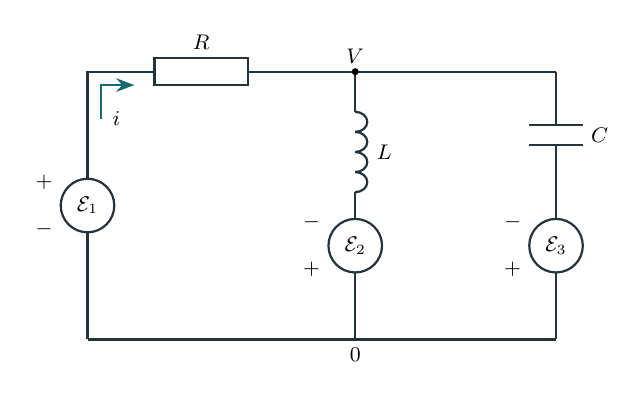
\begin{tikzpicture}[scale=.85,transform shape]

\draw[object] (0,0)--(0,1.6); \draw[object] (0,2.4)--(0,4)--(1,4);
\draw[object] (1,3.8) rectangle (2.4,4.2); \node[above] at (1.7,4.2) {$R$};
\draw[object] (2.4,4)--(7,4);
\draw[object] (0,0)--(7,0);
\draw[object] (0,2) circle (.4); \node at (0,2) {$\mathcal E_1$};
\node[left] at (-.4,2.35) {$+$};\node[left] at (-.4,1.65) {$-$};
\draw[object] (4,4)--(4,3.4);
\foreach \y in {3.4,3.1,2.8,2.5}{\draw[object] (4,\y) arc[start angle=90,end angle=-90,x radius=.18,y radius=.15];}
\node[right] at (4.2,2.8) {$L$};
\draw[object] (4,2.2)--(4,1.8); \draw[object] (4,1.4) circle (.4);
\draw[object] (4,1)--(4,0);
\node at (4,1.4) {$\mathcal E_2$};
\node[left] at (3.6,1.75) {$-$};\node[left] at (3.6,1.05) {$+$};
\draw[object] (7,4)--(7,3.2); \draw[object] (6.6,3.2)--(7.4,3.2);
\draw[object] (6.6,2.9)--(7.4,2.9); \draw[object] (7,2.9)--(7,1.8);
\node[right] at (7.4,3.05) {$C$};
\draw[object] (7,1.4) circle (.4); \node at (7,1.4) {$\mathcal E_3$};
\draw[object] (7,1)--(7,0);
\node[left] at (6.6,1.75) {$-$};\node[left] at (6.6,1.05) {$+$};
\draw[motion] (.2,3.3)--(.2,3.8)--(.7,3.8);
\node[right] at (.25,3.3) {$i$};
\fill (4,4) circle (1.5pt) node[above] {$V$};
\node[below] at (4,0) {$0$};

\end{tikzpicture}
\figcaption{图综一.4\quad 电源极性与电阻电流方向；三电源的频率依次为$\omega/2$、$\omega$、$2\omega$。}
\end{minipage}\end{center}

\Needspace{6\baselineskip}\subsection*{解答}


图综一.4中三个电源频率依次为$\omega/2$、$\omega$和$2\omega$。电路中的电阻、电感和电容均满足线性关系，电流可逐频率求出后在时域相加。保留一个电源时，其余理想电压源置零为短路，图中的上下节点及支路连接保持相同。以下相量的模取正弦量的峰值，记虚数单位为$\mathrm j$。

先用图中上节点$V$统一支路方向：设上节点电势相量为$V$，对应频率的电源相量为$E_1,E_2,E_3$，各不在本频率的电源置零。依图上极性，
\[
I=\frac{E_1-V}{R}
=\frac{V+E_2}{Z_L}+\frac{V+E_3}{Z_C}.
\]
中、右支路均取向下电流为正，$Z_L=\mathrm j\Omega L$、$Z_C=1/(\mathrm j\Omega C)$，每算一个频率都应重新代入$\Omega$。
\begin{center}\begin{minipage}{.98\linewidth}\centering
\begin{tikzpicture}[scale=.85,transform shape]

\node at (3.4,5.3) {$\Omega=\omega/2$，仅$\mathcal E_1$工作};
\draw[object] (0,0)--(0,4)--(1,4);
\draw[object] (1,3.8) rectangle (2.4,4.2); \node[above] at (1.7,4.2) {$R$};
\draw[object] (2.4,4)--(7,4); \draw[object] (0,0)--(7,0);
\draw[object] (4,4)--(4,3.4); \draw[object] (3.7,2.4) rectangle (4.3,3.4);
\node[right] at (4.3,2.9) {$ \mathrm jR/2 $};
\draw[object] (4,2.4)--(4,0);
\draw[object] (7,4)--(7,3.4); \draw[object] (6.7,2.4) rectangle (7.3,3.4);
\node[right] at (7.3,2.9) {$ -2\mathrm jR $}; \draw[object] (7,2.4)--(7,0);
\draw[motion] (0,3.3)--(0,3.7)--(.6,3.7); \node[left] at (0,3.3) {$I_1$};
\fill[white] (-0.09,.8) rectangle (0.09,1.8);\draw[object] (0,1.3) circle (.5);\node at (0,1.3) {$E_1$};\node[left] at (-0.5,1.7) {$+$};\node[left] at (-0.5,.9) {$-$};
\end{tikzpicture}
\figcaption{解图综一.4A\quad 低频分量：电阻串联LC并联阻抗。}
\end{minipage}\end{center}
三个电源分别激励的回路虽有不同的串并联组合，其节点式可统一整理为
\[
D=\frac1R+\frac1{Z_L}+\frac1{Z_C},\qquad
V=\frac{E_1/R-E_2/Z_L-E_3/Z_C}{D}.
\]
例如低频时$D=(1-3\mathrm j/2)/R$，节点电压等于$E_1/(1-3\mathrm j/2)$，代入$I_1=(E_1-V)/R$便得到图A的电流。高频时$D=(1+3\mathrm j/2)/R$，节点电压由右支路的$-E_3/Z_C$项决定，电阻电流向上返回为$-V/R$。这两个方向与图A、C的箭头相同。

解图综一.4A对应$\Omega=\omega/2$，仅保留$\mathcal E_1$。此时
\[
Z_L=\frac{\mathrm jR}{2},\qquad Z_C=-2\mathrm jR,
\qquad
Z_{LC}=\frac{Z_LZ_C}{Z_L+Z_C}=\frac{2\mathrm jR}{3}.
\]
电源看到$R+Z_{LC}=R(1+2\mathrm j/3)$，电阻电流为
\[
I_1=\frac{E_0e^{\mathrm j30^\circ}}{R(1+2\mathrm j/3)}
=\frac{3E_0}{\sqrt{13}R}
e^{\mathrm j[30^\circ-\arctan(2/3)]}.
\]
所以
\[
i_1(t)=\frac{3E_0}{\sqrt{13}R}
\cos\left(\frac{\omega t}{2}+30^\circ-\arctan\frac23\right).
\]
该分量电流滞后自身电源$\arctan(2/3)$，相位约$-3.69^\circ$。
\begin{center}\begin{minipage}{.98\linewidth}\centering
\begin{tikzpicture}[scale=.85,transform shape]

\node at (3.4,5.3) {$\Omega=\omega$，仅$\mathcal E_2$工作};
\draw[object] (0,0)--(0,4)--(1,4);
\draw[object] (1,3.8) rectangle (2.4,4.2); \node[above] at (1.7,4.2) {$R$};
\draw[object] (2.4,4)--(7,4); \draw[object] (0,0)--(7,0);
\draw[object] (4,4)--(4,3.4); \draw[object] (3.7,2.4) rectangle (4.3,3.4);
\node[right] at (4.3,2.9) {$ \mathrm jR $};
\draw[object] (4,2.4)--(4,0);
\draw[object] (7,4)--(7,3.4); \draw[object] (6.7,2.4) rectangle (7.3,3.4);
\node[right] at (7.3,2.9) {$ -\mathrm jR $}; \draw[object] (7,2.4)--(7,0);
\draw[motion] (0,3.3)--(0,3.7)--(.6,3.7); \node[left] at (0,3.3) {$I_2$};
\fill[white] (3.91,.8) rectangle (4.09,1.8);\draw[object] (4,1.3) circle (.5);\node at (4,1.3) {$E_2$};\node[left] at (3.5,1.7) {$-$};\node[left] at (3.5,.9) {$+$};
\end{tikzpicture}
\figcaption{解图综一.4B\quad 中频分量：内部电源通过电感及R、C并联返回，电阻电流非零。}
\end{minipage}\end{center}
解图综一.4B对应$\Omega=\omega$，仅保留$\mathcal E_2$。电感与中间电源串联，外部回路由$R$和$C$并联构成。沿中间电源升压方向取向下电流$J_2$，
\[
Z_{R\parallel C}=\frac{R(-\mathrm jR)}{R-\mathrm jR}
=\frac R2(1-\mathrm j),\qquad
Z_{\rm total}=\frac R2(1+\mathrm j).
\]
于是
\[
J_2=\frac{E_0e^{\mathrm j45^\circ}}{(R/2)(1+\mathrm j)}
=\frac{\sqrt2 E_0}{R}.
\]
并联部分向上返回的电阻电流按导纳分流：
\[
I_2=J_2\frac{Z_C}{R+Z_C}
=J_2\frac{1-\mathrm j}{2}
=\frac{E_0}{R}e^{-\mathrm j45^\circ}.
\]
因此
\[
i_2(t)=\frac{E_0}{R}\cos(\omega t-45^\circ).
\]
在$\Omega=\omega$时，$1/Z_L+1/Z_C=0$，节点方程化为$-V/R=E_2/Z_L$。图B的中间电源与电感串联，$E_2/Z_L$驱动电流沿电感支路向下，再由左侧电阻向上返回。于是$V=\mathrm jE_2$，$I_2=-V/R=-\mathrm jE_2/R$，与分流步骤给出的相位一致。
\begin{center}\begin{minipage}{.98\linewidth}\centering
\begin{tikzpicture}[scale=.85,transform shape]

\node at (3.4,5.3) {$\Omega=2\omega$，仅$\mathcal E_3$工作};
\draw[object] (0,0)--(0,4)--(1,4);
\draw[object] (1,3.8) rectangle (2.4,4.2); \node[above] at (1.7,4.2) {$R$};
\draw[object] (2.4,4)--(7,4); \draw[object] (0,0)--(7,0);
\draw[object] (4,4)--(4,3.4); \draw[object] (3.7,2.4) rectangle (4.3,3.4);
\node[right] at (4.3,2.9) {$ 2\mathrm jR $};
\draw[object] (4,2.4)--(4,0);
\draw[object] (7,4)--(7,3.4); \draw[object] (6.7,2.4) rectangle (7.3,3.4);
\node[right] at (7.3,2.9) {$ -\mathrm jR/2 $}; \draw[object] (7,2.4)--(7,0);
\draw[motion] (0,3.3)--(0,3.7)--(.6,3.7); \node[left] at (0,3.3) {$I_3$};
\fill[white] (6.91,.8) rectangle (7.09,1.8);\draw[object] (7,1.3) circle (.5);\node at (7,1.3) {$E_3$};\node[left] at (6.5,1.7) {$-$};\node[left] at (6.5,.9) {$+$};
\end{tikzpicture}
\figcaption{解图综一.4C\quad 高频分量：电容与内部电源串联，再经R、L并联返回。}
\end{minipage}\end{center}
解图综一.4C对应$\Omega=2\omega$，仅保留$\mathcal E_3$。此时
\[
Z_L=2\mathrm jR,\qquad Z_C=-\frac{\mathrm jR}{2},
\]
\[
Z_{R\parallel L}=\frac{2\mathrm jR}{1+2\mathrm j}
=\frac R5(4+2\mathrm j),
\quad Z_{\rm total}=Z_{R\parallel L}+Z_C=\frac R{10}(8-\mathrm j).
\]
取向下通过右电源的电流$J_3$，其电阻返回分流为
\[
\begin{aligned}
I_3&=\frac{E_0e^{\mathrm j60^\circ}}{(R/10)(8-\mathrm j)}
\frac{2\mathrm j}{1+2\mathrm j}\\
&=\frac{E_0}{R}\frac{4(3+2\mathrm j)}{13}e^{\mathrm j60^\circ}\\
&=\frac{4E_0}{\sqrt{13}R}
e^{\mathrm j[60^\circ+\arctan(2/3)]}.
\end{aligned}
\]
故高频分量相位约$93.69^\circ$。三者相加，
\[
\boxed{\begin{aligned}
i(t)=\frac{E_0}{R}\bigg[
&\frac3{\sqrt{13}}\cos\left(\frac{\omega t}{2}
+30^\circ-\arctan\frac23\right)\\
&+\cos(\omega t-45^\circ)\\
&+\frac4{\sqrt{13}}\cos\left(2\omega t
+60^\circ+\arctan\frac23\right)\bigg].
\end{aligned}}
\]
\begin{center}\begin{minipage}{.98\linewidth}\centering
\begin{tikzpicture}[scale=.85,transform shape]

\draw[axis] (0,0)--(7,0) node[right] {$\Omega/(\omega/2)$};
\draw[axis] (0,0)--(0,4) node[above] {$I_{\rm peak}/(E_0/R)$};
\draw[traj] (1.4,0)--(1.4,2.496); \fill (1.4,2.496) circle (2pt);
\draw[traj] (2.8,0)--(2.8,3); \fill (2.8,3) circle (2pt);
\draw[traj] (5.6,0)--(5.6,3.328); \fill (5.6,3.328) circle (2pt);
\node[below] at (1.4,0) {$1$};\node[below] at (2.8,0) {$2$};\node[below] at (5.6,0) {$4$};
\node[above] at (1.4,2.496) {$3/\sqrt{13}$};
\node[above] at (2.8,3) {$1$};
\node[above] at (5.6,3.328) {$4/\sqrt{13}$};
\node at (3.4,-1.4) {$T_0=4\pi/\omega,\quad\langle i_n i_m\rangle=0\ (n\ne m)$};

\end{tikzpicture}
\figcaption{解图综一.4D\quad 以共同周期平均，三个不同频率分量的交叉项为零。}
\end{minipage}\end{center}
解图综一.4D以共同基频$\omega/2$标出三条谱线，谐波序数为$1,2,4$。共同周期是$T_0=4\pi/\omega$。不同序数的正弦函数在完整共同周期内正交，具体地
\[
\frac1{T_0}\int_0^{T_0}
\cos(n\Omega_0t+\phi_n)\cos(m\Omega_0t+\phi_m)\,dt=0
\quad(n\ne m),
\]
将乘积写成和差形式，积分中的角频率分别为$(n-m)\Omega_0$与$(n+m)\Omega_0$；在$T_0=2\pi/\Omega_0$内，两个角度都增加整数个$2\pi$，首末正弦值相等，故积分为零。例如低频与中频的乘积为
\[
\cos(\Omega_0t+\phi_1)\cos(2\Omega_0t+\phi_2)
=\tfrac12\cos(\Omega_0t+\phi_2-\phi_1)
+\tfrac12\cos(3\Omega_0t+\phi_1+\phi_2).
\]
其中$\Omega_0=\omega/2$，本题$n,m\in\{1,2,4\}$；同频平方平均为$1/2$。所以
\[
\begin{aligned}
\bar P&=R\langle i^2\rangle
=\frac R2\left[\frac{9E_0^2}{13R^2}
+\frac{E_0^2}{R^2}+\frac{16E_0^2}{13R^2}\right]\\
&=\boxed{\frac{19E_0^2}{13R}}.
\end{aligned}
\]
上述平均取完整共同周期，瞬时功率由$P(t)=Ri(t)^2$给出。给定初始电感电流和电容电压时，稳态解加上衰减暂态便可满足两个储能元件的初始条件；经过足够长时间，电阻功率的时间平均趋向上式。
三个平方项各自贡献的平均功率依次为
\[
\bar P_1=\frac{9E_0^2}{26R},\qquad
\bar P_2=\frac{E_0^2}{2R},\qquad
\bar P_3=\frac{8E_0^2}{13R}.
\]
图D的谱线高度是峰值电流，平均功率由各高度的平方乘$R/2$得到。因而高频分量对平均发热的贡献最大，中频分量的平均功率占总值的$13/38$。



\Needspace{13\baselineskip}

\pdfbookmark[2]{第 5 题 幂律径向电场中的粒子束聚焦}{q5}

\section*{第 5 题\quad 幂律径向电场中的粒子束聚焦}\label{q:5}


平面内有径向电场$\boldsymbol E=-\kappa r^{-\beta}\hat{\boldsymbol r}$，其中$\kappa>0$、$\beta\ne1$。质量$m$、正电荷$q$的粒子从$S$发射，不计粒子间作用、重力和辐射。
\begin{enumerate}
\item 粒子以切向速度$v_0$沿半径$r_0$的圆轨道运动，求$r_0$。
\item 发射速率均为$v_0$，方向相对圆轨道切线有小角度偏离：最外射线偏外$\alpha_{\rm out}$，最内射线偏内$\alpha_{\rm in}$，总角宽$\alpha=\alpha_{\rm out}+\alpha_{\rm in}\ll1$。求使粒子在距中心$r_0$处重新聚焦的$\beta$范围、第一次聚焦的方位角$\phi_1$，以及方位角$\phi_1/2$处的径向束宽。取$\beta=-13$，画出粒子从$S$到转过$2\pi$的轨迹示意。
\item 在上述可聚焦范围内，改为方向均沿切线，速率分布在$v_0$至$v_0+\Delta v$，其中$\Delta v/v_0\ll1$。求第一次聚焦角$\phi_2$及方位角$\phi_2/2$处径向束宽；同样画$\beta=-13$时的轨迹。
\end{enumerate}
聚焦位置和束宽均求小角度、小相对速度差的一阶近似，说明稳定性和近似条件。


\begin{center}\begin{minipage}{.98\linewidth}\centering
\begin{tikzpicture}[scale=.8,transform shape]

\draw[object] (0,0) circle (2.5);
\fill (0,0) circle (2pt) node[below left] {$O$};
\fill (2.5,0) circle (2pt) node[below right] {$S$};
\draw[guide] (0,0)--(2.5,0) node[midway,below] {$r_0$};
\draw[motion] (2.5,0)--(2.5,2) node[above] {$v_0$切向};
\draw[motion] (2.5,0)--(3.1,1.9);
\draw[motion] (2.5,0)--(1.9,1.9);
\draw[force] (1.77,1.77)--(.85,.85) node[midway,above left] {$q\boldsymbol E$};
\draw[axis] (.8,0) arc[start angle=0,end angle=55,radius=.8];
\node at (.95,.5) {$\theta$};
\node[align=left] at (6,.4) {（2）小角宽$\alpha$\\（3）切向速度展宽$\Delta v$\\$\boldsymbol E=-\kappa r^{-\beta}\hat{\boldsymbol r}$};

\end{tikzpicture}
\figcaption{图综一.5\quad 参考圆、径向电力与两种发射展宽条件。}
\end{minipage}\end{center}

\Needspace{6\baselineskip}\subsection*{解答}


图综一.5的中心$O$指向发射点$S$，$OS=r_0$，参考粒子在$S$沿正方位角方向作切向运动。圆轨道条件为
\[
q\kappa r_0^{-\beta}=\frac{mv_0^2}{r_0},
\qquad
\boxed{r_0=\left(\frac{q\kappa}{mv_0^2}\right)^{1/(\beta-1)}}.
\]
题设取$\beta\ne1$，圆轨道条件据此唯一确定$r_0$。作为对照，$\beta=1$时同一条件变为$q\kappa=mv_0^2$，速度固定后，各半径均满足圆轨道条件。

圆轨道也是径向运动的参考平衡位置。对图中的切向发射稍作改变，粒子便在半径方向偏离参考圆。中央力对$O$的力矩为零，因此偏离过程中角动量守恒；半径增加时，角速度随之减小。径向恢复作用由电场力与角动量固定时的离心项共同决定，比较它们对半径的变化率，就能确定偏离是往复振动还是逐渐增大。方向展宽与速度展宽虽然都造成径向偏离，它们改变的初始量不同：前者在一阶内只给出径向初速度，后者还改变切向角动量，使每条射线的平衡位置外移。

令$\omega_0=v_0/r_0$，先把这一径向机制写成时间方程。对角动量为$h_0=r_0^2\omega_0$的粒子，置$r=r_0+x$，则
\[
\dot\theta=\frac{h_0}{r^2}
=\omega_0(1+x/r_0)^{-2}
=\omega_0(1-2x/r_0)+O(x^2/r_0^2).
\]
径向动力学方程$m\ddot r=mr\dot\theta^2-q\kappa r^{-\beta}$中的两项分别展开为
\[
\begin{aligned}
mr\dot\theta^2&=m\omega_0^2r_0(1+x/r_0)(1-4x/r_0)+O(x^2)
=m\omega_0^2r_0(1-3x/r_0)+O(x^2),\\
q\kappa r^{-\beta}&=q\kappa r_0^{-\beta}(1-\beta x/r_0)+O(x^2)
=m\omega_0^2r_0(1-\beta x/r_0)+O(x^2).
\end{aligned}
\]
常数项相消后，剩下
\[
\ddot x+(3-\beta)\omega_0^2x=0.
\]
其中$3$来自角动量守恒所决定的$h_0^2/r^3$项，$\beta$来自电场力随半径的变化。$\beta<3$时，向外偏离产生向内的合力，向内偏离产生向外的合力，径向运动为小振动。振动角频率与参考圆角速度之比为$\sqrt{3-\beta}$，它将直接决定轨迹在一周内交回参考圆的次数。

为把不同粒子的轨迹在同一方位角比较，使用比耐方程。比耐方程把时间换成方位角，可直接比较图上同一径向线穿过的多条射线。由$u=1/r$、$\dot\theta=hu^2$得
\[
\dot r=-hu',\qquad
\ddot r=-h^2u^2u'',\qquad
r\dot\theta^2=h^2u^3.
\]
将它们代入$\ddot r-r\dot\theta^2=-(q\kappa/m)r^{-\beta}$，除以$-h^2u^2$，便得到下面的轨道方程。因而这一步使用的仍是前述径向动力学和角动量守恒，只是把聚焦位置直接写成$\theta$的函数。
记单位质量角动量$h=r^2\dot\theta$、$u=1/r$，中央加速度为$-(q\kappa/m)r^{-\beta}$，于是
\[
u''+u=\frac{q\kappa}{mh^2}u^{\beta-2},
\]
撇号表示对$\theta$求导。圆轨道有$u_0=1/r_0$、$h_0=r_0v_0$，且
$(q\kappa/mh_0^2)u_0^{\beta-2}=u_0$。
\begin{center}\begin{minipage}{.98\linewidth}\centering
\begin{tikzpicture}[scale=.8,transform shape]

\draw[object] (0,0) circle (2.5);
\draw[guide] (2.5,-.8)--(2.5,3);
\draw[guide] (0,0)--(4,0) node[right] {径向外};
\fill (0,0) circle (2pt) node[below] {$O$};
\fill (2.5,0) circle (2pt) node[below right] {$S$};
\draw[motion] (2.5,0)--(3.4,2.3) node[above] {$\delta=\alpha_{\rm out}$};
\draw[motion] (2.5,0)--(1.6,2.3) node[above left] {$\delta=-\alpha_{\rm in}$};
\node[right] at (2.55,1) {$\delta$};
\node[align=left] at (6,-1) {$h=h_0+O(\delta^2)$\\$\dot r(0)=v_0\delta$\\$r-r_0\propto\sin(\eta\theta)$};

\end{tikzpicture}
\figcaption{解图综一.5A\quad 方向展宽一阶保留径向初速度，切向角动量的一阶变化为零。}
\end{minipage}\end{center}
第（2）问，解图综一.5A中初射方向与切线夹角$\delta$，偏外为正，偏内为负。由于$\cos\delta=1+O(\delta^2)$，一阶内$h=h_0$，径向初速度则保留$v_0\delta$。这两个初始条件分别进入轨道方程的系数和初斜率。
令$u=u_0+\zeta$，对比耐方程线性展开：
\[
\zeta''+\zeta=(\beta-2)\zeta
\ \Longrightarrow\ 
\zeta''+(3-\beta)\zeta=0.
\]
初始$\zeta(0)=0$。又由$\dot r=-h u'$，
\[
\zeta'(0)=-\frac{v_0\delta}{h_0}=-u_0\delta.
\]
若$\beta<3$，记$\eta=\sqrt{3-\beta}>0$，得
\[
\zeta=-\frac{u_0\delta}{\eta}\sin\eta\theta,\qquad
\boxed{r(\theta)=r_0+\frac{r_0\delta}{\eta}\sin\eta\theta
+O(\delta^2)}.
\]
所以第一次所有小角射线重新到达$r=r_0$且同一方位角处，是
\[
\boxed{\phi_1=\frac{\pi}{\sqrt{3-\beta}}}.
\]
在$\theta=\phi_1/2$处，正弦为一，最外和最内射线的径向偏移分别为$r_0\alpha_{\rm out}/\eta$和$-r_0\alpha_{\rm in}/\eta$，径向全束宽
\[
\boxed{\Delta r_1=\frac{\alpha r_0}{\sqrt{3-\beta}}}.
\]
聚焦点按相同方位角比较各条空间轨迹。取带符号的初始偏角 $\delta$，比角动量 $h=r_0v_0\cos\delta=r_0v_0+O(\delta^2)$。用解图综一.5B 中 $r/r_0=1+(\delta/4)\sin4\theta$ 的一阶轨迹，记 $\omega_0=v_0/r_0$，得到
\[
\frac{\mathrm dt}{\mathrm d\theta}=\frac{r^2}{h}
=\frac{1}{\omega_0}\left(1+\frac{\delta}{2}\sin4\theta\right)+O(\delta^2/\omega_0).
\]
从发射角 $0$ 积到 $\theta$，一阶到达时间比参考圆上的 $\theta/\omega_0$ 多 $\delta(1-\cos4\theta)/(8\omega_0)$。在奇数倍 $\pi/4$ 的焦点，正负偏角粒子经过同一地点，时间差是一阶量；在偶数倍 $\pi/4$ 的焦点，一阶时间差为零。

若$\beta=3$，扰动方程为$\zeta''=0$，非零初斜率引起线性漂移；若$\beta>3$，其解含$\sinh(\sqrt{\beta-3}\theta)$，也不重新为零。因此在题设$\beta\ne1$下，可聚焦范围为
\[
\boxed{\beta\in(-\infty,3)\setminus\{1\}}.
\]
等价的时间域径向小振动频率为
$\Omega_r=\sqrt{3-\beta}\,v_0/r_0$。靠近$\beta=3$时，径向恢复作用减弱，束宽中出现$1/\eta$放大因子；相应的小振动条件为$\alpha/\eta\ll1$，即展开后的$|r-r_0|/r_0$仍为小量。
\begin{center}\begin{minipage}{.98\linewidth}\centering
\begin{tikzpicture}[scale=.8,transform shape]

\draw[guide] (0,0) circle (3);
\foreach \a in {-.24,-.12,.12,.24}{
\draw[traj,domain=0:360,samples=361] plot ({(3+\a*sin(4*\x))*cos(\x)},{(3+\a*sin(4*\x))*sin(\x)});
}
\foreach \ang in {0,45,...,315}{\fill (\ang:3) circle (2pt);}
\fill (0,0) circle (2pt) node[below] {$O$};
\node[right] at (3.2,0) {$S$};
\node[above] at (0,3.3) {$\beta=-13,\quad\eta=4$};
\node at (0,-4) {每隔$\pi/4$交参考圆；径向偏移放大};

\end{tikzpicture}
\figcaption{解图综一.5B\quad 方向束的一阶轨迹，包含S在内的8个位置每周重复聚焦。}
\end{minipage}\end{center}
解图综一.5B取$\beta=-13$，$\eta=4$，轨迹一阶为
$r=r_0+(r_0\delta/4)\sin4\theta$。因此每隔$\pi/4$在参考圆上有一个聚焦点，离开$S$后，在$0<\theta\le2\pi$内共发生8次再聚焦，第8次回到$S$。内、外偏转两族在各焦点前后交换径向次序。

第（3）问改用切向速度$v=v_0(1+\epsilon)$发射，其中$\epsilon=(v-v_0)/v_0$。从时间域也能看清图C中平衡位置移动的大小。速度提高后$h=r_0v_0(1+\epsilon)$，径向方程中的离心项增加，而电场在出发点保持原值。一阶展开给出
\[
\begin{aligned}
\ddot x&=\frac{v_0^2}{r_0}(1+2\epsilon)(1-3x/r_0)
-\frac{v_0^2}{r_0}(1-\beta x/r_0)\\
&=2\epsilon\omega_0^2r_0-(3-\beta)\omega_0^2x.
\end{aligned}
\]
以$\eta^2=3-\beta$记回复系数，恒定驱动使平衡位置变为$x_{\rm eq}=2r_0\epsilon/\eta^2$。令$X=x-x_{\rm eq}$，则$\ddot X+\eta^2\omega_0^2X=0$。粒子从$r_0$切向射出，故$x(0)=\dot x(0)=0$，即$X(0)=-x_{\rm eq}$、$\dot X(0)=0$，振幅恰为$x_{\rm eq}$。沿图C从左到右，四分之一振动周期到平衡位置，半周期到最外侧$r_0+2x_{\rm eq}$，一整周期回到$r_0$。不同速度对应不同$x_{\rm eq}$，而一阶振动频率相同，因此第一次共同回到出发半径发生在整周期之后。

方向束则从$x=0$出发，初始径向速度分别为$v_0\alpha_{\rm out}$与$-v_0\alpha_{\rm in}$。其两侧振幅分别为$v_0\alpha_{\rm out}/\Omega_r$和$v_0\alpha_{\rm in}/\Omega_r$，所以半程的全束宽取两振幅之和。这个几何意义解释了$\alpha=\alpha_{\rm out}+\alpha_{\rm in}$进入结果的方式，切线在发散角内的偏置由两侧各自承担。

第（3）问，用$\epsilon=(v-v_0)/v_0\in[0,\Delta v/v_0]$。初始径向速度为零，但角动量已改变：
\[
h=h_0(1+\epsilon),\qquad
\frac1{h^2}=\frac1{h_0^2}(1-2\epsilon)+O(\epsilon^2).
\]
将$u=u_0+\zeta$和此式同时代入比耐方程，保留一阶项：
\[
\zeta''+(3-\beta)\zeta=-2u_0\epsilon,
\qquad \zeta(0)=\zeta'(0)=0.
\]
解为
\[
\zeta=-\frac{2u_0\epsilon}{\eta^2}(1-\cos\eta\theta),
\]
从而
\[
\boxed{r(\theta)=r_0+
\frac{2r_0\epsilon}{3-\beta}
[1-\cos(\sqrt{3-\beta}\theta)]+O(\epsilon^2)}.
\]
\begin{center}\begin{minipage}{.98\linewidth}\centering
\begin{tikzpicture}[scale=.8,transform shape]

\draw[axis] (0,0)--(8,0) node[right] {$\theta$};
\draw[axis] (0,0)--(0,4) node[above] {$r-r_0$};
\draw[guide] (0,1.5)--(7.2,1.5) node[right] {$x_{\rm eq}$};
\draw[traj,domain=0:360,samples=160] plot ({\x/50},{1.5*(1-cos(\x))});
\draw[guide] (3.6,0)--(3.6,3);
\node[below] at (3.6,0) {$\pi/\eta$};
\node[below] at (7.2,0) {$2\pi/\eta$};
\draw[axis,<->] (4.2,0)--(4.2,3);
\node[above] at (4.2,3.15) {$2x_{\rm eq}$};
\node at (3.8,4.7) {速度展宽：平衡位置外移，完整振动后回到$r_0$};

\end{tikzpicture}
\figcaption{解图综一.5C\quad 单条较快射线的径向偏移；最快粒子的$2x_{\rm eq}$即半程全束宽。}
\end{minipage}\end{center}
解图综一.5C画出恒定偏移和平移后的振动。较快粒子先偏向外侧；它的小振动中心相对参考圆外移
$x_{\rm eq}=2r_0\epsilon/(3-\beta)$，各条射线围绕各自的$r_0+x_{\rm eq}$振动。
第一次不同速率粒子都回到$r_0$需要余弦重新等于一，故
\[
\boxed{\phi_2=\frac{2\pi}{\sqrt{3-\beta}}=2\phi_1}.
\]
在$\phi_2/2$处余弦为$-1$，最慢参考粒子仍在$r_0$，最快粒子达到最大外偏，径向全束宽
\[
\boxed{\Delta r_2=
\frac{4r_0}{3-\beta}\frac{\Delta v}{v_0}}.
\]
速度束的小振动条件为$\Delta v/[(3-\beta)v_0]\ll1$。上述展开对每个固定的$\beta$取小展宽。若场力随半径变化特别快，保证$(1+|\beta|)|x|/r_0\ll1$即可使幂律展开中的高阶项保持很小。
\begin{center}\begin{minipage}{.98\linewidth}\centering
\begin{tikzpicture}[scale=.8,transform shape]

\draw[guide] (0,0) circle (3);
\foreach \a in {.05,.10,.15}{
\draw[traj,domain=0:360,samples=361] plot ({(3+\a*(1-cos(4*\x)))*cos(\x)},{(3+\a*(1-cos(4*\x)))*sin(\x)});
}
\foreach \ang in {0,90,180,270}{\fill (\ang:3) circle (2.5pt);}
\fill (0,0) circle (2pt) node[below] {$O$};
\node[right] at (3.25,0) {$S$};
\node[above] at (0,3.5) {$\beta=-13,\quad\phi_2=\pi/2$};
\node at (0,-4.1) {较快射线均在圆外；径向偏移放大};

\end{tikzpicture}
\figcaption{解图综一.5D\quad 速度束的一阶轨迹，每隔$\pi/2$回到参考圆，一周4次。}
\end{minipage}\end{center}
解图综一.5D中$\beta=-13$，速度束轨迹为
\[
r=r_0+\frac{r_0\epsilon}{8}(1-\cos4\theta),
\quad
\phi_2=\frac\pi2,\quad
\Delta r_2=\frac{r_0\Delta v}{4v_0}.
\]
它们均在参考圆外侧或圆上，每隔$\pi/2$聚焦，一周4次；这与方向展宽的一周8次不同。上述图线保留偏角和相对速度差的一阶项。有限展宽的轨迹还含二阶项，焦点附近的实际束斑可由继续展开轨道方程求出；这里的聚焦角和束宽描述一阶聚焦。


\Needspace{13\baselineskip}

\pdfbookmark[2]{第 6 题 列车入隧道与机械扰动的传播}{q6}

\section*{第 6 题\quad 列车入隧道与机械扰动的传播}\label{q:6}


隧道$A_1B_1$静止长度为$L_1$，列车$A_2B_2$自身静止长度为$L_2>L_1$。列车向左运动，$A_2$为前端，$B_2$为后端，隧道左端$A_1$是封闭挡墙，右端$B_1$设一扇门。
\begin{enumerate}
\item 选择速度$v$，使地面惯性系$S_1$中，前端$A_2$到达左墙$A_1$与后端$B_2$到达右门$B_1$两事件同时发生，求$v$。
\item 在列车碰撞前的静止惯性系$S_2$中，上述哪一事件先发生？两事件的时间间隔$\Delta t_2$是多少？即使列车后来发生碰撞，也继续使用这个惯性系。
\item 门在$S_1$所述同时事件处关上。用一个理想传播模型描述碰撞：前端一碰墙便随墙向右运动，而使车体运动状态改变的机械扰动从前端向后端传播；在尚未受扰的列车惯性系$S_2$中，传播速度为$u>0$，后端在扰动到达前保持静止。要使门到达并关住后端不晚于扰动到达后端，$u$应满足什么上界？
\end{enumerate}
若进一步假设这种材料的$u$不随$v$及所选$L_2$改变，并要求对任意满足第（1）问的列车与隧道均成立，证明$u\leq c$。这里讨论扰动到达的因果条件，不要求求解车体的具体压缩过程。


\begin{center}\begin{minipage}{.98\linewidth}\centering
\begin{tikzpicture}[scale=.8,transform shape]

\draw[object] (0,1)--(0,-.2)--(6,-.2)--(6,1);
\node[above] at (0,1) {$A_1$墙};\node[above] at (6,1) {$B_1$门};
\draw[axis,<->] (0,-1)--(6,-1) node[midway,below] {$L_1$};
\draw[object] (0,.1) rectangle (6,.65);
\node[below left] at (0,.1) {$A_2$};
\node[below right] at (6,.1) {$B_2$};
\draw[motion] (3,1.8)--(1,1.8) node[left] {$v$};
\node[right] at (7,.5) {$S_1$中恰好同时容纳};
\node at (3,-2.5) {列车碰撞前静长$L_2>L_1$，运动方向向左};

\end{tikzpicture}
\figcaption{图综一.6\quad 地面系中两个端点相遇事件同时发生，图示运动长度为L1。}
\end{minipage}\end{center}

\Needspace{6\baselineskip}\subsection*{解答}


图综一.6中$S_1$的$x$向右，列车速度为$-v$。选前端碰左墙为事件$F$，令其坐标$t_1=0,x_1=0$。后端遇右门事件$G$按第（1）问同时发生，坐标$t_1=0,x_1=L_1$。

在$S_1$中，碰撞前匀速列车长度为$L_2/\gamma$，其中
$\gamma=1/\sqrt{1-v^2/c^2}$。要同时恰好容纳，
\[
\frac{L_2}{\gamma}=L_1,\qquad
\gamma=\frac{L_2}{L_1},\qquad
\boxed{v=c\sqrt{1-\left(\frac{L_1}{L_2}\right)^2}}.
\]
这里的运动长度在碰撞刚发生前测量。取$S_1$中的同一时刻，车头与车尾的坐标差为$L_2/\gamma$；该长度与两隧道端点的坐标差相同，给出同时相遇所需的速度。此后车头受撞，车内各处的运动随扰动依次改变。
\begin{center}\begin{minipage}{.98\linewidth}\centering
\begin{tikzpicture}[scale=.68,transform shape]

\draw[axis] (0,0)--(6,0) node[right] {$x_1$};
\draw[axis] (0,0)--(0,3) node[above] {$ct_1$};
\draw[object] (0,0)--(4,0);
\fill (0,0) circle (2pt) node[below left] {$F$};
\fill (4,0) circle (2pt) node[below] {$G$};
\node at (2,1.5) {$\Delta t_1=0,\quad\Delta x_1=L_1$};
\begin{scope}[xshift=8cm]
\draw[axis] (0,0)--(5.6,0) node[right] {$x_2$};
\draw[axis] (0,0)--(0,4) node[above] {$ct_2$};
\fill (0,0) circle (2pt) node[below left] {$F$};
\fill (4,2.4) circle (2pt) node[above right] {$G$};
\draw[guide] (0,2.4)--(4,2.4)--(4,0);
\node[left] at (0,2.4) {$\beta_vL_2$};
\node[below] at (4,0) {$L_2$};
\end{scope}

\end{tikzpicture}
\figcaption{解图综一.6A\quad 同一对端点事件经洛伦兹变换，列车惯性系中G发生较晚。}
\end{minipage}\end{center}
解图综一.6A标出地面同时的$F,G$与$S_2$中的时间差。由于$S_2$相对$S_1$速度为$-v$，洛伦兹变换为
\[
t_2=\gamma\left(t_1+\frac{vx_1}{c^2}\right),
\qquad x_2=\gamma(x_1+vt_1).
\]
将两事件分别代入：
\[
F:(t_2,x_2)=(0,0),\qquad
G:\left(\frac{\gamma vL_1}{c^2},\,\gamma L_1\right)
=\left(\frac{vL_2}{c^2},\,L_2\right).
\]
所以前端先碰墙。右门到达车尾的时间间隔为
\[
\boxed{\Delta t_2=\frac{vL_2}{c^2}=\frac{\beta_vL_2}{c}},
\qquad \beta_v=v/c,
\]
在图A左侧，两个事件位于同一条地面同时线上。右侧的$G$位于$F$上方，高差为$\beta_vL_2$；这就是$S_2$中先碰墙、后到门的时间差乘以$c$。

把图A右侧的时间差转成图B中的追及距离，可以直接看出门为何晚到。隧道在$S_2$中向右匀速运动，长度$L_1/\gamma=L_1^2/L_2$。以$F$为原点，在$t_2=0$时门位于$x_2=L_1^2/L_2$，还要前进$L_2-L_1^2/L_2$才到后端。除以图B中门的速度$v$，得到
\[
\Delta t_2=\frac{L_2-L_1^2/L_2}{v}
=\frac{L_2(1-1/\gamma^2)}{v}
=\frac{vL_2}{c^2}.
\]
\begin{center}\begin{minipage}{.98\linewidth}\centering
\begin{tikzpicture}[scale=.8,transform shape]

\draw[axis] (0,0)--(7,0) node[right] {$x_2$};
\draw[axis] (0,0)--(0,6.5) node[above] {$ct_2$};
\draw[object] (5,0)--(5,5);
\node[below] at (5,0) {后端$B_2$};
\draw[traj] (3.2,0)--(6.8,6);
\draw[guide] (0,0)--(3.6,6);
\draw[force] (0,0)--(5,5);
\node[right,text=accent] at (7.2,4.6) {门$B_1$};
\node[right,text=warm] at (7.2,5.5) {扰动：$u=c$};
\fill (0,0) circle (2pt) node[below left] {$F$};
\fill (5,3) circle (2.5pt) node[right] {$G$：门先到};
\fill (5,5) circle (2.5pt) node[left] {扰动后到};
\draw[guide] (0,3)--(5,3); \node[left] at (0,3) {$c\Delta t_2$};
\node at (3.1,-1.3) {$\beta_v=0.6$示例，$S_2$始终是同一惯性系};

\end{tikzpicture}
\figcaption{解图综一.6B\quad 门与扰动到达后端的时序比较；虚线为墙的世界线。}
\end{minipage}\end{center}
解图综一.6B在持续使用的惯性系$S_2$画后端世界线$x_2=L_2$、门的世界线及从$F$出发的扰动。扰动尚未到达后端时，后端静止，传播所需时间为
$t_{\rm sig}=L_2/u$。门不晚于扰动到达后端，要求
\[
\Delta t_2\leq\frac{L_2}{u}
\ \Longleftrightarrow\
\boxed{u\leq\frac{L_2}{\Delta t_2}
=\frac{c^2}{v}}.
\]
在图B的示例中，门与扰动依次到达车尾。对一般$u$，沿未受扰车尾的竖直线比较两条斜线的交点。门的交点在下方时门先到，两交点重合时同时到达。对固定$v<c$，从这条后端世界线读出的上界为$c^2/v$，大于$c$。

取图B的时间轴向上，墙和门两条世界线分别为
\[
x_{A_1}=vt_2,\qquad x_{B_1}=\frac{L_1^2}{L_2}+vt_2.
\]
从$F$出发的扰动前沿满足$x_{\rm sig}=ut_2$。在门到达的位置$x_2=L_2$处，前沿尚未越过后端的条件写成
\[
u\Delta t_2\leq L_2,\qquad
0<u\leq \frac{c}{\sqrt{1-(L_1/L_2)^2}}.
\]
左式比较的是门到达那一时刻的两个位置，与右面按到达时间写出的条件相同。$u$取到上界时两条斜线在后端世界线上交于同一点。对所有$v$使用同一个$u$时，图C中每个$v/c$横坐标都给出一个可取区间，各区间的公共部分为$0<u\leq c$。

进一步使用题设“$u$不随$v,L_2$改变，且对所有满足条件的组合均成立”。由于$L_2/L_1$可任意大，$v$可任意接近$c$，上界的下确界是
\[
\inf_{0<v<c}\frac{c^2}{v}=c,\qquad
\boxed{u\leq c}.
\]
也可用反证明确“所有速度”的条件：若$u=a_0c$、$a_0>1$，可在$1<a<a_0$之间选一个$a$，取$v=c/a<c$，并相应选择
\[
L_2=\frac{L_1}{\sqrt{1-1/a^2}}>L_1.
\]
该组合满足第（1）问，却有$u=a_0c>ac=c^2/v$，此时$L_2/u<\Delta t_2$，扰动到达点位于图B中门事件的下方，与题设到达顺序矛盾。
\begin{center}\begin{minipage}{.98\linewidth}\centering
\begin{tikzpicture}[scale=.85,transform shape]

\draw[axis] (0,0)--(6,0) node[right] {$v/c$};
\draw[axis] (0,0)--(0,5.8) node[above] {$u_{\max}/c$};
\draw[traj,domain=.2:1,samples=160] plot ({5*\x},{1/\x});
\draw[guide] (0,1)--(5.5,1); \node[left] at (0,1) {$1$};
\draw[guide] (5,0)--(5,1); \node[below] at (5,0) {$1$};
\draw[accent,fill=white] (5,1) circle (2pt);
\node[right] at (3.3,2.2) {$u_{\max}/c=1/(v/c)$};
\node at (3,-1.5) {对所有$v<c$均成立的共同上界为$c$};

\end{tikzpicture}
\figcaption{解图综一.6C\quad 给定速度的上界大于c；要求任意速度成立时取下确界。}
\end{minipage}\end{center}
解图综一.6C中，$v$越大，允许的$u$上界越接近$c$。在图B的碰撞模型里，前端从$F$起沿墙的世界线向右，扰动抵达车尾以前，后端保持在$x_2=L_2$，所以车身两端之间的距离逐渐缩短。门在这一时段到达车尾时，可按题设关门。$S_2$始终是同一惯性坐标系；车体各段受扰后的运动由各自世界线描述。


\end{document}
